%% LyX 1.6.2 created this file.  For more info, see http://www.lyx.org/.
%% Do not edit unless you really know what you are doing.
\documentclass[10pt,oneside,english]{book}
\usepackage{mathptmx}
\usepackage[T1]{fontenc}
\usepackage[latin9]{inputenc}
\usepackage[a4paper]{geometry}
\geometry{verbose,tmargin=3cm,bmargin=2cm,lmargin=3cm,rmargin=3cm,headheight=0.5cm,headsep=0.4cm,footskip=1cm}
\setcounter{secnumdepth}{3}
\setcounter{tocdepth}{3}
\usepackage{color}
\usepackage{float}
\usepackage{amsthm}
\usepackage{amsmath}
\usepackage{graphicx}


%%%%%%%%%%%%%%%%%%%%%%%%%%%%%% LyX specific LaTeX commands.
%% Because html converters don't know tabularnewline
\providecommand{\tabularnewline}{\\}
\floatstyle{ruled}
\newfloat{algorithm}{tbp}{loa}[chapter]
\floatname{algorithm}{Algorithm}

%%%%%%%%%%%%%%%%%%%%%%%%%%%%%% Textclass specific LaTeX commands.
\theoremstyle{plain}
\newenvironment{lyxcode}
{\par\begin{list}{}{
\setlength{\rightmargin}{\leftmargin}
\setlength{\listparindent}{0pt}% needed for AMS classes
\raggedright
\setlength{\itemsep}{0pt}
\setlength{\parsep}{0pt}
\normalfont\ttfamily}%
 \item[]}
{\end{list}}

\usepackage{babel}

\begin{document}

\title{Advances In Programming Languages: proceedings of the 2009 SICSA
summer school.}

\maketitle
\listof{algorithm}{List of Algorithms}


\listoffigures


\listoftables



\chapter{SIMD and Multi-core Parallelisation in an Imperative Language.}


\author{Paul Cockshott, Tamerlan Tajadinov}


\section{Hardware Context}



One of the most significant trends that can be observed in the modern
processor design is towards an increased parallelism. Single Instruction
Multiple Data-stream (SIMD) computing has a long history\cite{dap,hillis},
but in the 1990s, a technique that had previously only been applicable
in large machines began to be applied to microprocessors\cite{tremblay1996vis,peleg1996mmx}.
Primarily aimed at graphics applications, SIMD instructions were introduced
for the x86 in Pentium MMX processors allowing saturated arithmetic
to be performed on up to eight 8-bit or two 32-bit integers at a time.
The concept was further developed in SSE2 processors\cite{conte2000long}
by allowing floating point operations to be performed on up to four
single precision or two double precision floats at a time, while also
doubling the number of possible integer operands. The IBM/Sony Cell
\cite{kahle2005introduction}processor used in the PlayStation 3 also
operates on vectors of data of similar size. Moreover, the next generation
of Intel GPGPUs codenamed Larrabee also follows the trend by allowing
up to 64 8-bit integers or 16 single precision floats to be operated
on with a single instruction.

While traditionally an increase in the performance of a CPU used to
be associated with an increased clock speed, this historic trend is
no longer observed as much. An increase in the clock speed demands
a sharp increase in the power consumption and leads to a rise in the
heat dissipation, thus the clock speed is limited by reasons of thermodynamics
to presently around 3.5GHz as in case of Wolfdale DP generation of
Xeon processors. This limitation is now increasingly commonly compensated
for by planting multiple cores on a processor chip - a solution that
has originated from high performance systems the performance of which
frequently benefits from multiple CPUs. As the number of cores in
a system increases, the CPU clock speed tends to be reduced by the
processor designers, thus the 4-core Core 2 Quad processor operates
on frequencies of up to 3.2GHz depending on the model of the chip
compared to its single core predecessor Pentium 4 running on clock
speeds of up to 3.8GHz several years prior. In mobile computing demands
on reduced power consumption have retained CPU frequencies at much
lower rates of around 1-2.5GHz and dual and even quad core processors
are widely used.

The above developments in the topic of processor design have introduced
further demands in compiler design. The majority of imperative programming
languages, especially those derived from C, typically operate on a
single element at a time, thus, for example, should we wish to add
two vectors of integers together each pair of elements will be added
one at a time, which is not in line with the hardware capabilities
allowing for arithmetic operations to be performed on multiple operands
at a time. Furthermore, unless multiple threads are explicitly spawned,
only one of the cores is likely to be utilised, leading to the reducing
processor clock speed being the main performance indicator for applications
written in these legacy programming languages. The remainder of this
article discusses Vector Pascal, an imperative language designed to
utilise the increasing capacity of modern processors through hardware
parallelism.


\section{The Example Language}

Vector Pascal\cite{cockshottsigplan} was developed by the computer
vision group at the University of Glasgow as a language for high performance
image processing. It is an extension of Pascal\cite{jensen1991pum,ISO90a}
with array language concepts. Array programming languages arose from
the work of Iverson. During the 1950s, when the latter was working
as a doctoral student for the Nobelist Leontief on the computation
of the US input output tables he developed Iverson's Notation, a concise
and unambiguous mathematical notation for expressing matrix computation.
The notation was taken up by IBM and released as the computer language
APL\cite{iverson62}. What distinguished APL from other contemporary
languages was both its rather abstruse character set, and its ability
to concisely express calculations over whole arrays in a single assignment
statement. It was an untyped interpretive language. Pascal on the
other hand is famously a strongly typed language. There have been
many interpretive successors to APL, the most popular ones being Matlab\cite{mathworks1984matlab}
and J\cite{Jmanual}. Introduction of array language techniques into
typed imperative languages started with versions of FORTRAN\cite{dapfortran,Ewing,brainerd1996programmer}.
A number of other compiled array languages have subsequently been
developed\cite{Snyder,blelloch,GrelSchoPPL03}. What has distinguished
Vector Pascal from these is its particular emphasis on efficient targeting
the parallel features embodied in commodity microprocessors: initially
SIMD instructions, and more recently multi-core facilities. In what
follows we describe only those extended features of the language that
relate to parallelism. Extensions relating to the type system, mathematical
character sets etc, are ignored.


\subsection{Extend array semantics}

Standard Pascal allows assignment of whole arrays. Vector Pascal\cite{cockshottsigplan}
extends this to allow consistent use of mixed rank expressions on
the right hand side of an assignment. For example, given:
\begin{lyxcode}
r1:\textcolor{red}{array}{[}0..7{]}~\textcolor{red}{of~real};

r2:\textcolor{red}{array}{[}0..7,0..7{]}~\textcolor{red}{of~real}
\end{lyxcode}
then we can write: 
\begin{lyxcode}
\textrm{~~1.}~r1:=~1/2;~~\\
~\textrm{2.}~r2:=~r1{*}3;~~\\
~\textrm{3.}~r1:=~r1+r2{[}1{]};~
\end{lyxcode}

\subsection{Equivalent loops\label{sub:Equivalent-loops}}

Line 1 assigns \texttt{0.5} to each element of \texttt{r1}. 

Line 2 assigns \texttt{1.5} to every element of \texttt{r2}. 

In line 3, \texttt{r1} is incremented with the corresponding elements
of row 1 of \texttt{r2}. 

These are defined to be equivalent to the following standard Pascal
loops: 
\begin{lyxcode}
\textrm{1'.}~\textcolor{red}{for}~$\iota_{0}$:=0~\textcolor{red}{to}~7~\textcolor{red}{do}~

~~~~r1{[}$\iota_{0}${]}:=1/2;~~\\
\textrm{2'.}~\textcolor{red}{for}~$\iota_{0}$:=0~\textcolor{red}{to}~7~\textcolor{red}{do}~

~~~~\textcolor{red}{for}~$\iota_{1}$:=0~\textcolor{red}{to}~7~\textcolor{red}{do}~

~~~~~~r2{[}$\iota_{0},\iota_{1}${]}:=r1{[}$\iota_{1}${]}{*}3;~

\textrm{3'.}~~\textcolor{red}{for}~$\iota_{0}$:=0~\textcolor{red}{to}~7~\textcolor{red}{do}~

~~~~r1{[}$\iota_{0}${]}:=r1{[}$\iota_{0}${]}+r2{[}1,$\iota_{0}${]};~
\end{lyxcode}
The compiler has to generate an implicit loop\index{loop}. In the
above \texttt{$\iota_{0},\iota_{1}$,$t$} are temporary variables
created by the compiler. The implicit indices \texttt{$\iota_{0},\iota_{1}$}
etc are accessible to a coder using the syntax \texttt{iota{[}0{]},
iota{[}1{]}} etc. 


\subsection{Data reformatting}

Given two conforming matrices a, b

the statement
\begin{lyxcode}
a:=~\textcolor{red}{trans}~b;
\end{lyxcode}
will transpose the matrix b into a.

For more general reorganisations you can permute the implicit indices
thus
\begin{lyxcode}
a:=\textcolor{red}{perm}{[}1,0{]}~b~;

\{~equivalent~to~a:=~trans~b~\}



z:=\textcolor{red}{perm}{[}1,2,0{]}~y;
\end{lyxcode}
In the second case z and y must be 3 d arrays and the result is such
that z{[}i,j,k{]}=y{[}j,k,i{]}. It is clearly desirable to do this
in a way which prevents the creation of temporary arrays. We will
discuss below the general strategy to minimise the creation of temporaries.

Given \texttt{\small a:}\texttt{\textcolor{red}{array}}\texttt{\small {[}0..10,0..15{]}
}\texttt{\textcolor{red}{of}}\texttt{\small{} t}; then 

\begin{tabular}{ll}
\texttt{\small a{[}1{]}} & \texttt{\textcolor{red}{array}}\texttt{\small{} {[}0..15{]}}\texttt{\textcolor{red}{
of}}\texttt{\small{} t}\tabularnewline
\texttt{\small a{[}1..2{]}} & \texttt{\textcolor{red}{array}}\texttt{\small{} {[}0..1,0..15{]}}\texttt{\textcolor{red}{
of}}\texttt{\small{} t}\tabularnewline
\texttt{\small a{[}{]}{[}1{]}} & \texttt{\textcolor{red}{array}}\texttt{\small {[}0..10,0..0{]} }\texttt{\textcolor{red}{of}}\texttt{\small{}
t}\tabularnewline
\texttt{\small a{[}1..2,4..6{]}} & \texttt{\textcolor{red}{array}}\texttt{\small {[}0..1,0..3{]} }\texttt{\textcolor{red}{of}}\texttt{\small{}
t}\tabularnewline
\end{tabular}


\subsection{Implicit mapping}

Maps are implicitly defined on both operators and functions. 

If \texttt{f} is a function or unary operator mapping from type $T_{1}$
to type $T_{2}$ and \texttt{x} : \texttt{\textcolor{red}{array of}}
$T_{1}$ then \texttt{a:=f(x)} assigns an array of $T_{2}$ such that
\texttt{a{[}i{]}=f(x{[}i{]})}. Similarly if we have \texttt{g(p,q:}$T_{1}$\texttt{):}
$T_{2}$,then \texttt{a:=g(x,y)} for \texttt{x,y:}\texttt{\textcolor{red}{array
of}} $T_{1}$ gives \texttt{a{[}i{]}=g(x{[}i{]},y{[}i{]})}


\subsection{Pixel Arithmetic}

Pixels are a predefined data type, represented as 8 bit signed fixed
point binary fractions. The numerical range of pixels is from -1 to
+1. Arithmetic on pixels is inherently saturating. The existence of
types supporting saturated arithmetic is an advantage in image processing.


\section{Parsing and Automatic Mapping of Operators and Functions\label{sec:Parsing-and-Automatic}}

Translation takes place using a modification of the classic single
pass compiler approach used by Wirth\cite{jensen1991pum}, and described
in \cite{davie1982recursive}. In this approach a recursive recognising
function is declared for each non-terminal in the grammar of the source
language. On success the recognising function outputs, as a side effect,
a stream of byte codes for a machine independent intermediate code.
We have modified the approach in two ways in both order to parse array
expressions and also to allow the efficient translation of the array
expressions to parallel code.

\begin{tabular}{ccccc}
 & compiler &  & code generator & \tabularnewline
 &  & tree-form &  & machine\tabularnewline
pascal source & $\rightarrow$ & intermediate & $\rightarrow$ & specific\tabularnewline
 &  & code &  & assembler\tabularnewline
\end{tabular}

Since the work of Budd\cite{Budd} it has been known that efficient
compilation of an array language requires that one eliminate the formation
of temporary arrays in the course of array expressions. It turns out
that a simple extension of recursive descent parsing techniques allows
this.

Consider a simplified version of the Vector Pascal grammar for assignments
:
\begin{lyxcode}
<ass>~~~::=~<variable>~':='~<exp>

<exp>~~~::=~<term><addop><term>

<term>~~::=~<factor><multop><factor>

<factor>::=~'('~<exp>~')'~

~~~~~~~~|~<variable>

~~~~~~~~|~<reduction>~<factor>

~~~~~~~~|~'trans'~<factor>
\end{lyxcode}
Consider the following example produced by the grammar:
\begin{lyxcode}
z:=~y+~\textbackslash{}+(A~{*}~B~);
\end{lyxcode}
where \texttt{y,z} are vectors and \texttt{A, B} matrices. \textbackslash{}
is the reduction functional which reduces an expression by an operator.
Thus \textbackslash{}+ forms the sum along the rows of the matrix
formed by the Hadamard product of \texttt{A} and \texttt{B}. A naive
compilation would generate 3 temporaries for this, a matrix for \texttt{A{*}B},
a vector for the sum of \texttt{A{*}B} then a final vector as a result
of adding y.

A standard recursive descent parser would have functions \texttt{ass,
exp, term, factor : typedescriptor} which would read the compiler
input stream, return the type of the expression or sub expression
they recognised, and as a side-effect output a stream of intermediate
byte-codes. In order to handle array expressions we modify these so
that they are now of the form:
\begin{lyxcode}
function~exp(Iotalocations:vector):IlcgTree;
\end{lyxcode}
Each parsing function now takes as a parameter a vector of addresses
of memory locations to be used as loop index variables, and instead
of returning a type, it returns a intermediate code tree. The assignment
function inspects its first symbol - a variable and determines the
rank of the variable. It then creates a vector of index locations
with respect to the current frame pointer and passes this vector in
to the call it makes on exp. The length of the vector of index locations
is determined by the rank of the variable being assigned to. The following
pseudo code explains the technique:
\begin{lyxcode}
function~ass:IlcgTree;

~~musthave(Id\_symbol);

~~id:=currentsymbol;r:=rankof(id);

~~v:=~createIotaVector(r);

~~e:=~exp(v);

~~dest:=~locationof(id);

~~for~i~:=~1~to~r~do

~~~~dest:=~subscript(dest,v{[}i{]});

~~return~createnestedforloops(dest,v,e);
\end{lyxcode}
To understand what is produced refer back to section \ref{sub:Equivalent-loops}.
The exp function in turn passes the vector of index locations to its
terms:
\begin{lyxcode}
function~exp(Iotalocations:vector):IlcgTree;

~~t1:=~term(Iotalocations);

~~if~have~(~addop~)~then

~~~~~op:=currentsymbol;

~~~~~t2:=term(Iotalocations)

~~~~~return~dyad(t1,op,t2)

~~else~return~t1;
\end{lyxcode}
At the bottom level of the parse, the function to recognise a variable
uses the index vector to reduce any array variable to a scalar. 
\begin{lyxcode}
function~variable(Iotalocations:vector):IlcgTree;

~~musthave(Id\_symbol);

~~id:=currentsymbol;

~~r:=getrank(id);

~~u:=upbound(Iotalocations);

~~v:=~locationof(id);

~~for~i~:=~1~to~r~do

~~~~v:=~subscript(v,iotalocation{[}i+u-r{]});

~~return~v;


\end{lyxcode}
The \texttt{subscript} function constructs and returns an intermediate
code tree to perform the subscription of the variable by the contents
of the memory location described by \texttt{Iotalocations}. The effect
is that the exp function will always return intermediate code that
will evaluate to a scalar rather than an array. This scalar result
is then embedded in a for loop as specified in section \ref{sub:Equivalent-loops}.
All intermediate array values are eliminated allowing the code generator
to use conventional register optimisation techniques for array valued
expressions. There are a couple of special cases worth noting:
\begin{enumerate}
\item Reduction factors. On encountering a reduction functional the \texttt{factor}
function creates a new vector of indices. If the initial vector of
\texttt{Iotalocations} was of length n this will be of length n+1
with the last element being the address of a new index variable to
be used in a reduction loop. This longer vector of indices is then
passed into a recursive call of \texttt{factor}. The code generated
for the reduction is always for a scalar operation. 
\item Transpositions and permutations. These are performed on the index
vector at compile time before passing it in to a recursive call of
the \texttt{factor} parsing function. There is no additional run time
cost associated with the transpose operation.
\end{enumerate}
The vector of index locations is similar in principle to the technique
used in Single Assignment C \cite{GrelSchoPPL03} for array de-referencing,
but whereas in SAC an index vector is explicitly present in the indexing
semantics of the language, in our case it is an implicit vector existing
only at compile time. Vector Pascal allows the index vector \texttt{iota}
to be used in sub-scripted form within a factor thus
\begin{lyxcode}
p:=~q{[}iota{[}0{]}+1{]}{*}0.5+q{[}iota{[}0{]}-1{]}{*}0.5;
\end{lyxcode}
would be legal where 
\begin{lyxcode}
p:array{[}1..n{]}~of~real;q:~array{[}0..n+1{]}~of~real;
\end{lyxcode}
but it do not allow \texttt{iota} to be passed as a parameter to a
function, or allow it to be indexed by a run time expression. Although,
in simple cases, \texttt{iota} corresponds to a sequence of ascending
adjacent addresses, and could thus be mapped to a conventional array,
in more complex expressions involving matrix transpositions or reduction
operations this is no longer true.


\section{Opportunities to Parallelise Array Assignments}

Explain why SIMD code is particularly appropriate for vectors or for
the 2nd dimension of matrices. Explain why multi core can readily
operate on 1st dimension of matrices. Explain the best assignment
of processors to rows of the matrix -- doing alternate rows instead
of the first half then the 2nd half. == Tamerlan


\section{Transformation for SIMD Parallelism}

The intermediate code generated by the parser described in section
\ref{sec:Parsing-and-Automatic} produces scalar serialised intermediate
code. This can be run on any processor, but if the processor has vector
registers the scalar code will be sub-optimal. After the parser has
generated code for an assignment it queries the code generator to
see if vector registers are available for the data type produced by
the expression. If yes, then the scalar intermediate code is a candidate
to be transformed to vectorised intermediate code. We will illustrate
the process of translating code for array expressions with an ultra-simple
example which adds two images together. When operating with 8 bit
pixels one has the problem that arithmetic operations can wrap round.
Thus adding two bright pixels can lead to a result that is dark. So
one has to put in guards against this. The problem of adding two arrays
of pixels and making sure that we never get any pixels wrapping round
can be solved in C a shown in Algorithm \ref{alg:C-code-to}.

%
\begin{algorithm}


\caption{C code to add two images, along with timing on a 3Ghz Opteron. Compiled
with gcc.\label{alg:C-code-to}}

\begin{lyxcode}
{\footnotesize \#define~LEN~6400}{\footnotesize \par}

{\footnotesize \#define~CNT~100000}{\footnotesize \par}

{\footnotesize main()}{\footnotesize \par}

{\footnotesize \{}{\footnotesize \par}

{\footnotesize{}~~unsigned~char~v1{[}LEN{]},v2{[}LEN{]},v3{[}LEN{]};}{\footnotesize \par}

{\footnotesize{}~~int~i,j,t;}{\footnotesize \par}

{\footnotesize{}~/{*}~repeat~many~times~for~timing~{*}/}{\footnotesize \par}

{\footnotesize{}~~for(i=0;i<CNT;i++)}{\footnotesize \par}

{\footnotesize{}~~~~~for~(j=0;j<LEN;j++)~{[}}{\footnotesize \par}

{\footnotesize{}~~~~~~t=v2{[}j{]}+v1{[}j{]};}{\footnotesize \par}

{\footnotesize{}~~~~~~if(~t>255)t=255;~}{\footnotesize \par}

{\footnotesize{}~~~~~~v3{[}j{]}=t;}{\footnotesize \par}

{\footnotesize{}~~~~~\}}{\footnotesize \par}

{\footnotesize \}}{\footnotesize \par}

{\footnotesize {[}wpc@maui~tests{]}\$~time~C/a.out}{\footnotesize \par}

{\footnotesize real~~~~0m2.854s}{\footnotesize \par}

{\footnotesize user~~~~0m2.813s}{\footnotesize \par}

{\footnotesize sys~~~~~0m0.004s}{\footnotesize \par}
\end{lyxcode}

\end{algorithm}
%
\begin{algorithm}
\caption{Vector Pascal \label{alg:Vector-Pascal-code}code equivalent to the
C code in Algorithm \ref{alg:C-code-to}. Timing on the same machine
as in Algorithm \ref{alg:C-code-to}.}

\begin{lyxcode}
\textcolor{red}{\footnotesize program}{\footnotesize{}~vecadd;}{\footnotesize \par}

\textcolor{red}{\footnotesize type}{\footnotesize{}~byte=0..255;}{\footnotesize \par}

\textcolor{red}{\footnotesize var}{\footnotesize{}~v1,v2,v3:}\textcolor{red}{\footnotesize array}{\footnotesize {[}0..6399{]}}\textcolor{red}{\footnotesize of}{\footnotesize{}~byte;}{\footnotesize \par}

{\footnotesize{}~~~~i:}\textcolor{red}{\footnotesize integer}{\footnotesize ;}{\footnotesize \par}

\textcolor{red}{\footnotesize begin}{\footnotesize \par}

{\footnotesize{}~~~~~}\textcolor{red}{\footnotesize for}{\footnotesize{}~i:=~1~}\textcolor{red}{\footnotesize to}{\footnotesize{}~100000~}\textcolor{red}{\footnotesize do}{\footnotesize{}~}{\footnotesize \par}

{\footnotesize{}~~~~~~~~~v3:=v1~+:~v2;}{\footnotesize \par}

{\footnotesize{}~~~~~~~~\{~}\textcolor{green}{\footnotesize +:~is~the~saturated~add~operation}{\footnotesize{}~\}}{\footnotesize \par}

\textcolor{red}{\footnotesize end}{\footnotesize .}{\footnotesize \par}

{\footnotesize {[}wpc@maui~tests{]}\$~time~vecadd}{\footnotesize \par}

{\footnotesize real~~~~0m0.094s}{\footnotesize \par}

{\footnotesize user~~~~0m0.091s}{\footnotesize \par}

{\footnotesize sys~~~~~0m0.005s}
\end{lyxcode}

\end{algorithm}


The equivalent Vector Pascal code is shown in Algorithm \ref{alg:Vector-Pascal-code}.
The very much improved performance comes from effective utilisation
of the available SIMD instructions on the Opteron. The original statement
is translated into ILCG as shown:


\paragraph*{Pascal}
\begin{lyxcode}
~~v3:=v1~+:~v2;
\end{lyxcode}

\paragraph*{ILCG}
\begin{lyxcode}


{\footnotesize{}~~~~~mem(ref~uint8~vector~(~6400~),~~+(PmainBase,~-25600)~):=}{\footnotesize \par}

{\footnotesize{}~~~~~+:(\textasciicircum{}(mem(ref~uint8~vector~(~6400~),~~+(PmainBase,~-12800))),}{\footnotesize \par}

{\footnotesize{}~~~~~~~~\textasciicircum{}(mem(ref~uint8~vector~(~6400~),~~+(PmainBase,~-19200)))))~}{\footnotesize \par}
\end{lyxcode}
Note that all operation are annotated with type information, and all
variables are resolved to explicit address calculations in ILCG. Hence
it is close to the machine, but it still allows expression of parallel
operations.\texttt{ }The symbol \texttt{\textasciicircum{}} is the
ILCG dereference operation, following the Pascal convention. Efficient
translation depends on there being a close match available between
the semantics of available machine instructions and the ILCG operations
specified by the first level of translation. We specify the machine
instruction-set in ILCG. As an example, here are some key instruction
specifications taken from the machine specification file \texttt{\footnotesize gnuPentium.ilc}
which specifies the semantics of the Gnu assembler language for the
Pentium:


\paragraph*{Saturated Add  Bytes}
\begin{lyxcode}
\textcolor{red}{\footnotesize instruction~pattern}{\footnotesize{}~PADDUSB(mreg~m,~mrmaddrmode~ma)~~~~~}{\footnotesize \par}

{\footnotesize{}~}\textcolor{red}{\footnotesize means}{\footnotesize {[}(ref~uint8~vector(8))m~:=~}{\footnotesize \par}

{\footnotesize{}~~~~~~(uint8~vector(8))+:((uint8~vector(8))\textasciicircum{}(m),}{\footnotesize \par}

{\footnotesize{}~~~~~~~~~~~~~~~~~~~~~~~~~~(uint8~vector(8))\textasciicircum{}(ma)){]}~~~~~~}{\footnotesize \par}

{\footnotesize{}~}\textcolor{red}{\footnotesize assembles}{\footnotesize{}~{[}'paddusb~'ma~','~m{]};}{\footnotesize \par}
\end{lyxcode}

\paragraph*{Vector Load and Store }
\begin{lyxcode}
\textcolor{red}{\footnotesize instruction~pattern}{\footnotesize{}~MOVQL(maddrmode~rm,~mreg~m)~~~~~~~~~}{\footnotesize \par}

{\footnotesize{}~~}\textcolor{red}{\footnotesize means}{\footnotesize {[}m~:=~(doubleword)\textasciicircum{}(rm){]}~~~}{\footnotesize \par}

{\footnotesize{}~~}\textcolor{red}{\footnotesize assembles}{\footnotesize {[}'movq~'~rm~','~m'\textbackslash{}n~prefetchnta~128+'rm{]};}{\footnotesize \par}

\textcolor{red}{\footnotesize instruction~pattern}{\footnotesize{}~MOVQS(maddrmode~rm,~mreg~m)~~~~~~~~~}{\footnotesize \par}

{\footnotesize{}~~}\textcolor{red}{\footnotesize means}{\footnotesize {[}(ref~doubleword)rm:=~\textasciicircum{}(m){]}~~~~~~~~}{\footnotesize \par}

{\footnotesize{}~~}\textcolor{red}{\footnotesize assembles}{\footnotesize {[}'movq~'m~','rm{]};}{\footnotesize \par}
\end{lyxcode}


We automatically build a family of optimising  code generators that
translate from ILCG trees to linear assembly code by pattern matching.

\begin{tabular}{ccccc}
 & ILCG  &  & Java  & \tabularnewline
 & Compiler &  & Compiler & \tabularnewline
Pentium.ilc & $\rightarrow$ & Pentium.java & $\rightarrow$ & Pentium.class\tabularnewline
Opteron.ilc & $\rightarrow$ & Opteron.java & $\rightarrow$ & Opteron.class\tabularnewline
\end{tabular}

To port to new machines one has to write a machine description of
that CPU in ILCG. We currently have production versions for the Intel
and AMD machines\cite{Jackson05} since the 386 plus Beta versions
for the PlayStation 2\cite{cooper05} and PlayStation 3.

Basic array operations are broken down into strides equal to the machine
vector length. Then these are then matched to machine instructions
following the general approach of Graham \cite{graham} to generate
code.

\emph{ILCG input to Opteron.class}
\begin{lyxcode}


{\footnotesize{}~~~~~mem(ref~uint8~vector~(~6400~),~~+(PmainBase,~-25600)~):=}{\footnotesize \par}

{\footnotesize{}~~~~~+:(\textasciicircum{}(mem(ref~uint8~vector~(~6400~),~~+(PmainBase,~-12800))),}{\footnotesize \par}

{\footnotesize{}~~~~~~~~\textasciicircum{}(mem(ref~uint8~vector~(~6400~),~~+(PmainBase,~-19200)))))~}{\footnotesize \par}
\end{lyxcode}
\emph{Assembler output by Opteron.class}
\begin{lyxcode}
{\footnotesize{}~~~leaq~~~~~~~~~0,\%rdx~~~~~~~~~~~~~;~init~loop~counter}{\footnotesize \par}

{\footnotesize l1:cmpq~~~~~~~~~\$~6399,~\%rdx}{\footnotesize \par}

{\footnotesize{}~~~jg~~~~~~~~~~~l3}{\footnotesize \par}

{\footnotesize{}~~~movq~~~~~~~~~PmainBase-12800(\%rdx),\%MM4}{\footnotesize \par}

{\footnotesize{}~~~prefetchnta~128+PmainBase-12800(\%rdx)~;~get~data~16~iterations~~}{\footnotesize \par}

{\footnotesize{}~~~~~~~~~~~~~~~~~~~~~~~~~~~~~~~~~~~~~~~~~;~~ahead~into~cache}{\footnotesize \par}

{\footnotesize{}~~~paddusb~~~~~PmainBase-19200(\%rdx),\%MM4}{\footnotesize \par}

{\footnotesize{}~~~movq~~~~~~~~\%MM4,PmainBase-25600(\%rdx)}{\footnotesize \par}

{\footnotesize{}~~~addq~~~~~~~~\$~8,\%rdx}{\footnotesize \par}

{\footnotesize{}~~~jmp~~~~~~~~~l1}{\footnotesize \par}

{\footnotesize l3:}{\footnotesize \par}
\end{lyxcode}
To maintain comparability with the C example we show the code generated
at optimisation level 0. The timing shown in Algorithm \ref{alg:Vector-Pascal-code}
was obtained at optimisation level 0. At higher optimisation levels
vectorisation is followed by loop unrolling and other well known techniques.
These result considerably more opaque assembler.


\subsection{Preconditions for SIMD parallelisation}

For SIMD parallelisation to be viable a number of conditions must
be checked.
\begin{enumerate}
\item The expression on the right hand side must not contain any function
calls, since functions return scalar results.
\item The operands in the expression must be of the same data length. For
instance, one can not efficiently perform SIMD addition between two
arrays if one contains 32 floating point numbers and the other contains
64 bit floating point.
\item The least significant indices of all arrays in the expression must
either be the same, or must differ by an additive term. Thus the ILCG
code equivalent to \texttt{a{[}i,j{]}+b{[}i,j{]}} is SIMD parallelisable
as is \texttt{a{[}i,j+10{]}+b{[}i,j{]}} but \texttt{a{[}i,j{]}+b{[}j,i{]}}
would not be parallelisable since in the case of \texttt{b} we are
stepping down columns as \texttt{j} is incremented. Since column elements
are not stored adjacently in memory, one can not perform a SIMD load
of them. Nor would \texttt{a{[}i,j{]}+b{[}i,j{*}3{]}} be parallelisable,
again because the successive elements of \texttt{b} being used are
not adjacent. On the other hand \texttt{a{[}i,j{]}+c{[}i{]}} for some
column vector \texttt{c} can be parallelised since it is usually possible
to replicate a scalar \texttt{c{[}i{]}} across all elements of a SIMD
register.
\item If the array lengths being operated on are not an integer multiple
of the SIMD register lengths, SIMD and scalar code must be combined.
Suppose the array length is 10 and the register length is 4. Then
SIMD code is used to operate on the first 8 elements of the array,
and scalar code for the remaining two elements. For dynamic arrays,
this test has to be delayed until run time. In this case the 'remainder
code' is performed by an optional scalar loop appended to the SIMD
loop.
\end{enumerate}

\section{Transformation for Multi-core Parallelism}

SIMD vectorisation works for one dimensional data, or on the last
dimension for arrays stored in row major order, because the hardware
has to work on adjacent words. SIMD gives considerable acceleration
on image data, and worthwhile accelerations on floating point and
integer data. Future machines like the Larrabee will have considerably
wider SIMD registers, increasing the benefits of SIMD code. But newer
chips also have multiple cores. For these, the recent versions of
the Vector Pascal compiler will parallelise across multiple cores
if the arrays being worked on are of rank 2. The Pascal source code
of the program remains the same independently of whether it is being
targeted at a simple sequential machine, a SIMD machine or a multi-core
SIMD machine. Targeting is done by flags passed to the compiler:
\begin{lyxcode}
vpc~sub2dex~-cpu486
\end{lyxcode}
would compile sub2dex.pas using purely sequential 32 bit instructions.
\begin{lyxcode}
vpc~sub2dex~-cpuOpteron
\end{lyxcode}
would compile the same file targeted to a 64 bit Opteron with 1 core
using the SIMD instructions in the Opteron instructionset.
\begin{lyxcode}
vpc~sub2dex~-cpuOpteron~-cores2
\end{lyxcode}
would compile the file to a 64 bit Opteron with 2 cores and SIMD instructions.
The compiler is implemented in Java so the selection of code generators
and compilation strategies is achieved by dynamically loading appropriate
compiler and code generator classes.

Let us now look at the transformations required to achieve this using
a trivial rank 2 array example in Algorithm \ref{alg:Example-of-combined}.
The example is not intended to be realistic or useful, only illustrative.
We assume that the code has been compiled for a dual core Opteron.

%
\begin{algorithm}
\caption{Example of combined mult-core and SIMD parallelism.\label{alg:Example-of-combined}}

\begin{lyxcode}
\textcolor{red}{\footnotesize procedure}{\footnotesize{}~sub2d;}{\footnotesize \par}

\textcolor{red}{\footnotesize type}{\footnotesize{}~range=0..127;~}{\footnotesize \par}

\textcolor{red}{\footnotesize var}{\footnotesize{}~x,y,z:}\textcolor{red}{\footnotesize array}{\footnotesize {[}range,range{]}~}\textcolor{red}{\footnotesize of~real}{\footnotesize ;}{\footnotesize \par}

\textcolor{red}{\footnotesize begin}{\footnotesize \par}

{\footnotesize{}~~~~~~~~x:=y-z;}{\footnotesize \par}

\textcolor{red}{\footnotesize end}{\footnotesize ;}{\footnotesize \par}
\end{lyxcode}
This translates into ILCG as follows when compiled for a dual core
Opteron
\begin{lyxcode}
\textcolor{red}{\footnotesize procedure}{\footnotesize (sub2d,}{\footnotesize \par}

{\footnotesize{}~}\textcolor{red}{\footnotesize procedure}{\footnotesize{}~(label12~}\textcolor{green}{\footnotesize ...~see~Algorithm~\ref{alg:The-function-performing}}{\footnotesize{}~)}{\footnotesize \par}

{\footnotesize{}~post\_job{[}label12,\textasciicircum{}(\%rbp),1{]};~~~/{*}~}\textcolor{green}{\footnotesize send~to~core~1}{\footnotesize{}~{*}/}{\footnotesize \par}

{\footnotesize{}~/{*}~Note~that~\%rbp~is~the~Opteron~stack~frame~pointer~{*}/~~~~~~~~~~}{\footnotesize \par}

{\footnotesize{}~post\_job{[}label12,\textasciicircum{}(\%rbp),0{]};~~~/{*}~}\textcolor{green}{\footnotesize send~to~core~0}{\footnotesize{}~{*}/~~~~~~~~~~~~~}{\footnotesize \par}

{\footnotesize{}~wait\_on\_done{[}0{]};}{\footnotesize \par}

{\footnotesize{}~wait\_on\_done{[}1{]};}{\footnotesize \par}

{\footnotesize )}{\footnotesize \par}
\end{lyxcode}

\end{algorithm}


Two threads are dispatched to process the work using a fork - rejoin
paradigm. The run time library is built on top of pthreads\cite{nichols1996pthreads}.
For a two core machine, two server threads are initiated at program
start up. These wait on a semaphore until post\_job passes them the
address of a procedure and a stack frame context within which the
procedure is to be executed.

The statement x:=y-z  is translated into a procedure that can run
as a separate task, the ILCG has been simplified for comprehensibility
in Algorithm \ref{alg:The-function-performing}.

%
\begin{algorithm}
\caption{The function performing nested loops.\label{alg:The-function-performing}}

\begin{lyxcode}
\textcolor{red}{\scriptsize procedure}{\scriptsize{}~(label12~/{*}~}\textcolor{green}{\scriptsize internal~label}{\scriptsize {*}/~,}{\scriptsize \par}

{\scriptsize{}~}\textcolor{red}{\scriptsize for}{\scriptsize (mem(+(\textasciicircum{}(\%rbp),-24)),\textasciicircum{}(mem(+(\textasciicircum{}(\%rbp),16))),127~~,~~~}\textbf{\textcolor{blue}{\scriptsize 2}}{\scriptsize ,~}{\scriptsize \par}

{\scriptsize{}~~~~~/{*}}\textcolor{green}{\scriptsize iota~{[}0{]}~~~~~~~~~~~~~task~number~~~~~~~~limit~~step}{\scriptsize {*}/}{\scriptsize \par}

{\scriptsize{}~~}\textcolor{red}{\scriptsize var}{\scriptsize (mem(+(\textasciicircum{}(\%rbp),-32))),/{*}~iota{[}1{]}~{*}/}{\scriptsize \par}

{\scriptsize{}~~}\textcolor{red}{\scriptsize for}{\scriptsize (mem(+(\textasciicircum{}(\%rbp),-32)),~0~~~~,127,~~~~~}\textbf{\textcolor{blue}{\scriptsize 4}}{\scriptsize{}~,}{\scriptsize \par}

{\scriptsize{}~~~~~/{*}}\textcolor{green}{\scriptsize iota~{[}1{]}~~~~~~~~~~~~start~limit~~step}{\scriptsize {*}/}{\scriptsize \par}

{\scriptsize{}~~~mem(ref~ieee32~vector~(~4~),~/{*}~}\textcolor{green}{\scriptsize x{[}iota{[}0{]},iota{[}1{]}{]}}{\scriptsize{}~{*}/}{\scriptsize \par}

{\scriptsize{}~~~~~~~+(+({*}(\textasciicircum{}(mem(+(\textasciicircum{}(\%rbp),-24))),512),~}{\scriptsize \par}

{\scriptsize{}~~~~~~~~~+({*}(\textasciicircum{}(mem(+(\textasciicircum{}(\%rbp),-32))),~~4),-131072)),~}{\scriptsize \par}

{\scriptsize{}~~~~~~~~~~~\textasciicircum{}(mem(+(\textasciicircum{}(\%rbp),-8))))):=}{\scriptsize \par}

{\scriptsize{}~~~~~-(\textasciicircum{}(mem(ref~ieee32~vector~(~4~),/{*}~}\textcolor{green}{\scriptsize y{[}iota{[}0{]},iota{[}1{]}{]}}{\scriptsize{}~{*}/}{\scriptsize \par}

{\scriptsize{}~~~~~~~+(+({*}(\textasciicircum{}(mem(+(\textasciicircum{}(\%rbp),-24))),512),~}{\scriptsize \par}

{\scriptsize{}~~~~~~~~~+({*}(\textasciicircum{}(mem(+(\textasciicircum{}(\%rbp),-32))),~~4),-196608)),~}{\scriptsize \par}

{\scriptsize{}~~~~~~~~~~~\textasciicircum{}(mem(+(\textasciicircum{}(\%rbp),-8)))))),}{\scriptsize \par}

{\scriptsize{}~~~~~~~\textasciicircum{}(mem(ref~ieee32~vector~(~4~),/{*}~}\textcolor{green}{\scriptsize z{[}iota{[}0{]},iota{[}1{]}{]}}{\scriptsize{}~{*}/}{\scriptsize \par}

{\scriptsize{}~~~~~~~~~+(+({*}(\textasciicircum{}(mem(+(\textasciicircum{}(\%rbp),~-24))),512),~}{\scriptsize \par}

{\scriptsize{}~~~~~~~~~~~+({*}(\textasciicircum{}(mem(+(\textasciicircum{}(\%rbp),~-32))),~~4),-262144)),~}{\scriptsize \par}

{\scriptsize{}~~~~~~~~~~~~~\textasciicircum{}(mem(+(\textasciicircum{}(\%rbp),-8))))))))),}{\scriptsize \par}

{\scriptsize{}~)}
\end{lyxcode}

\end{algorithm}

\begin{lyxcode}
{\scriptsize{}~~~~~~}~~~~~~~~~~~~~~~
\end{lyxcode}
The basic structure of the task procedure is two nested for loops,
one for each dimension of the arrays. 

The outer loop or row index steps by 2 to ensure that each task will
process every 2nd row, starting at the row given by the task number.
Thus task 0 will process rows 0,2,4,6,... Task 1 will proocess rows
1,3,5,7,... If there are 4 cores available each task will process
every 4th row, etc. 

The inner loop, for the column indices, advances by 4 since the Opteron
has SIMD registers capable of handling 4 floating point numbers at
a time.


\section{The PURE Function Extension}

We define a pure function to be such that does not have any side effects,
i.e. it does not update any global, or shared, states outside of its
own scope. If the other functions are called from the body of the
function, these also have to be pure even if not marked as such. This
definition of pure functions is consistent with the definition used
in FORTRAN 95. Given the absence of explicit multi-threading constructs
in the given language, the above property of pure functions implies
thread safety. A function can be labeled as pure by prepending the
keyword \texttt{pure} in front of every declaration or definition
of the function. This means that if, for example, a function is declared
as pure in the interface section of the programme, it must be also
declared as pure anywhere else in the code, e.g. in the subsequent
definition of the function body. Any inconsistency in the declared
purity of a function is spotted by the compiler and treated as a syntactic
error.
\begin{lyxcode}
\textbf{pure}~\textbf{function}~next(i~:~integer):~integer;

\textbf{begin}

~~~~~~~~next~:=~i+1;

\textbf{end};
\end{lyxcode}
Above function \emph{next} operates only on the parameter passed to
it, thus it is appropriate to declare it as pure. The keyword \emph{pure}
does not bare any semantic value, other than it serves as a hint to
the compiler which may then generate multi-threaded code. Multi-threaded
code will be generated if -cores\emph{n} flag is passed to the compiler
specifying more than one core, and hence the number of threads, available
to the programme and if the function is then invoked as part of an
assignment statement.


\section{Task Parallelism and Block Structure}

The technique of procedurising code shown in Algorithms \ref{alg:Example-of-combined}
and \ref{alg:The-function-performing} is well established when parallelising
loops in Open-MP \cite{dagum1998openmp}. There are two significant
differences. First, and least significantly, in Vector Pascal the
loop is implicit rather than the explicit loops used in Open-MP. But
secondly Open-MP is targeted at C and FORTRAN which are flat languages.
Pascal is a block structured language which makes the access to variables
by spawned tasks somewhat more complex. Consider Algorithm \ref{alg:Taylor-series-example.}
which illustrates the use of nested blocks in Pascal. This has a main
program \texttt{nestpar} and embedded within that a procedure \texttt{emap}
which takes a matrix $a$ as a parameter and replaces each $a_{i,j}$
with $e^{scale.a_{i,j}}$ where $scale$ is a global variable. The
exponential function is approximated by a Taylor series 

\[
e^{x}=1+\frac{1}{1!}x^{1}+\frac{1}{1!}x^{1}+\frac{1}{2!}x^{2}+\frac{1}{3!}x^{3}+...\]


using the function \texttt{Taylor}. The Taylor series is evaluated
as

{\textsf{\textit{Taylor}$\leftarrow$  $\sum$  (\textit{coefs} $\times$ \textit{x}$^{\iota_{0}}$) }; } 

where $\iota_{0}=0,1,2,3...$ using the line
\begin{lyxcode}
Taylor:=~~~\textbackslash{}+~(coefs~{*}~x~pow~iota{[}0{]});
\end{lyxcode}
The coefs vector has been initialised in the main program to contain
the inverse factorial series as required.

%
\begin{algorithm}
\label{alg:Taylor-series-example.}\caption{Taylor series example.}

\begin{lyxcode}
{\footnotesize program~nestpar;}{\footnotesize \par}

{\footnotesize type~t~=~array{[}1..3,1..2{]}~of~real;}{\footnotesize \par}

{\footnotesize{}~~~~~coef=array{[}0..5{]}~of~real;}{\footnotesize \par}

{\footnotesize{}~~~~~~~~~~~~~~~~\{~tabulate~inverse~factorials~\}}{\footnotesize \par}

{\footnotesize const~expc:coef=(1,1,1/2,1/6,1/24,1/(5{*}24));}{\footnotesize \par}

{\footnotesize var~scale:real;B:t;}{\footnotesize \par}

{\footnotesize procedure~emap(var~a:t);}{\footnotesize \par}

{\footnotesize{}~~\{~for~each~a{[}i,j{]}~replace~with~a{[}i,j{]}+exp(scale{*}a{[}i,j{]})~\}}{\footnotesize \par}

{\footnotesize{}~~var~coefs:coef;}{\footnotesize \par}

{\footnotesize{}~~pure~function~Taylor(~x:real):real;}{\footnotesize \par}

{\footnotesize{}~~begin}{\footnotesize \par}

{\footnotesize{}~~~~Taylor:=~~~\textbackslash{}+~(coefs~{*}~x~pow~iota{[}0{]});}{\footnotesize \par}

{\footnotesize{}~~end;}{\footnotesize \par}

{\footnotesize begin}{\footnotesize \par}

{\footnotesize{}~~~coefs:=~expc;}{\footnotesize \par}

{\footnotesize{}~~~a~:=~Taylor(a{*}scale);}{\footnotesize \par}

{\footnotesize end;}{\footnotesize \par}

{\footnotesize begin}{\footnotesize \par}

{\footnotesize{}~~~~~scale:=0.1;}{\footnotesize \par}

{\footnotesize{}~~~~~B:=~iota{[}0{]}{*}iota{[}1{]};}{\footnotesize \par}

{\footnotesize{}~~~~~write(B);}{\footnotesize \par}

{\footnotesize{}~~~~~emap(B);}{\footnotesize \par}

{\footnotesize{}~~~~~write(B);}{\footnotesize \par}

{\footnotesize end.}{\footnotesize \par}
\end{lyxcode}
Output Produced
\begin{lyxcode}
{\footnotesize{}~~~~~1.00000~~~~~2.00000}{\footnotesize \par}

{\footnotesize{}~~~~~2.00000~~~~~4.00000}{\footnotesize \par}

{\footnotesize{}~~~~~3.00000~~~~~6.00000}{\footnotesize \par}

{\footnotesize{}~~~~~~~}{\footnotesize \par}

{\footnotesize{}~~~~~1.10517~~~~~1.22140}{\footnotesize \par}

{\footnotesize{}~~~~~1.22140~~~~~1.49182}{\footnotesize \par}

{\footnotesize{}~~~~~1.34986~~~~~1.82205}
\end{lyxcode}

\end{algorithm}


%
\begin{figure}
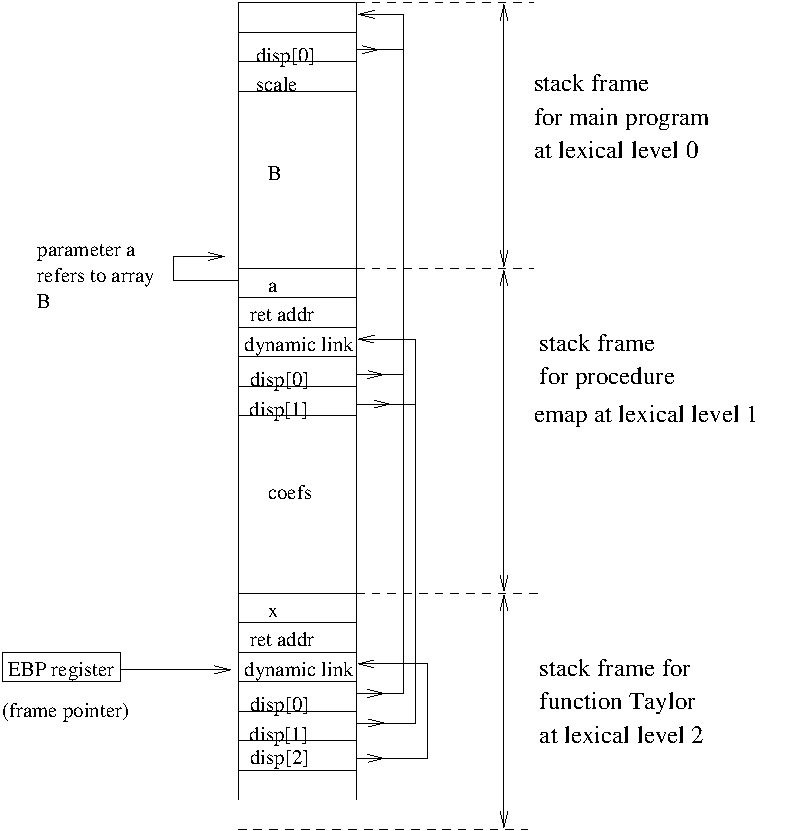
\includegraphics[scale=0.5]{nestparstack1}

\caption{Stack for nestpar in single core mode.\label{fig:Stack-for-nestpar}}



\end{figure}


There are a number of references from inner to outer scopes: \texttt{Taylor}
uses the vector \texttt{coefs}, and \texttt{emap} uses the variable
\texttt{scale}. There are three well known techniques for implementing
this in normal procedural code: $\lambda$lifting, static chaining
or display vectors. Since Intel provide direct hardware support for
display vectors in the procedure ENTER and LEAVE instructions we have
chosen to use displays. Figure \ref{fig:Stack-for-nestpar} illustrates
how the stack would be organised during execution of Taylor when the
program is compiled for a single core machine. Observe how Taylor
can access variables in the enclosing stack frames using the display
vector. But if the code is to run on a dual core machine there will
be not one but three stacks as shown in Figure \ref{fig:The-3-stacks}:
one for the main program and one each for the child tasks. The original
function \texttt{emap} will have been written to ILCG equivalent to:
\begin{lyxcode}
{\footnotesize procedure~emap(var~a:t);}{\footnotesize \par}

{\footnotesize{}~~var~coefs:coef;}{\footnotesize \par}

{\footnotesize{}~~pure~function~Taylor(~x:real):real;}{\footnotesize \par}

{\footnotesize{}~~begin}{\footnotesize \par}

{\footnotesize{}~~~~Taylor:=~~~\textbackslash{}+~(coefs~{*}~x~pow~iota{[}0{]});}{\footnotesize \par}

{\footnotesize{}~~end;}{\footnotesize \par}

{\footnotesize{}~~procedure~dummy(start:int);}{\footnotesize \par}

{\footnotesize{}~~var~iota:array{[}0..1{]}~of~integer;}{\footnotesize \par}

{\footnotesize{}~~begin}{\footnotesize \par}

{\footnotesize{}~~~~iota{[}0{]}:=start;}{\footnotesize \par}

{\footnotesize{}~~~~while~iota{[}0{]}<=3~do}{\footnotesize \par}

{\footnotesize{}~~~~begin}{\footnotesize \par}

{\footnotesize{}~~~~~~for~iota{[}1{]}:=1~to~2~do}{\footnotesize \par}

{\footnotesize{}~~~~~~~a{[}iota{[}0{]},iota{[}1{]}{]}:=Taylor(a{[}iota{[}0{]},iota{[}1{]}{]}{*}scale);}{\footnotesize \par}

{\footnotesize{}~~~~~~iota{[}0{]}:=iota{[}0{]}+2;}{\footnotesize \par}

{\footnotesize{}~~~~end;}{\footnotesize \par}

{\footnotesize{}~~end;}{\footnotesize \par}

{\footnotesize begin}{\footnotesize \par}

{\footnotesize{}~~~coefs:=~expc;}{\footnotesize \par}

{\footnotesize{}~~~post\_job(dummy,1);post\_job(dummy,0);}{\footnotesize \par}

{\footnotesize{}~~~wait\_on\_done(0);wait\_on\_done(1);}{\footnotesize \par}

{\footnotesize end;}{\footnotesize \par}
\end{lyxcode}
%
\begin{figure}
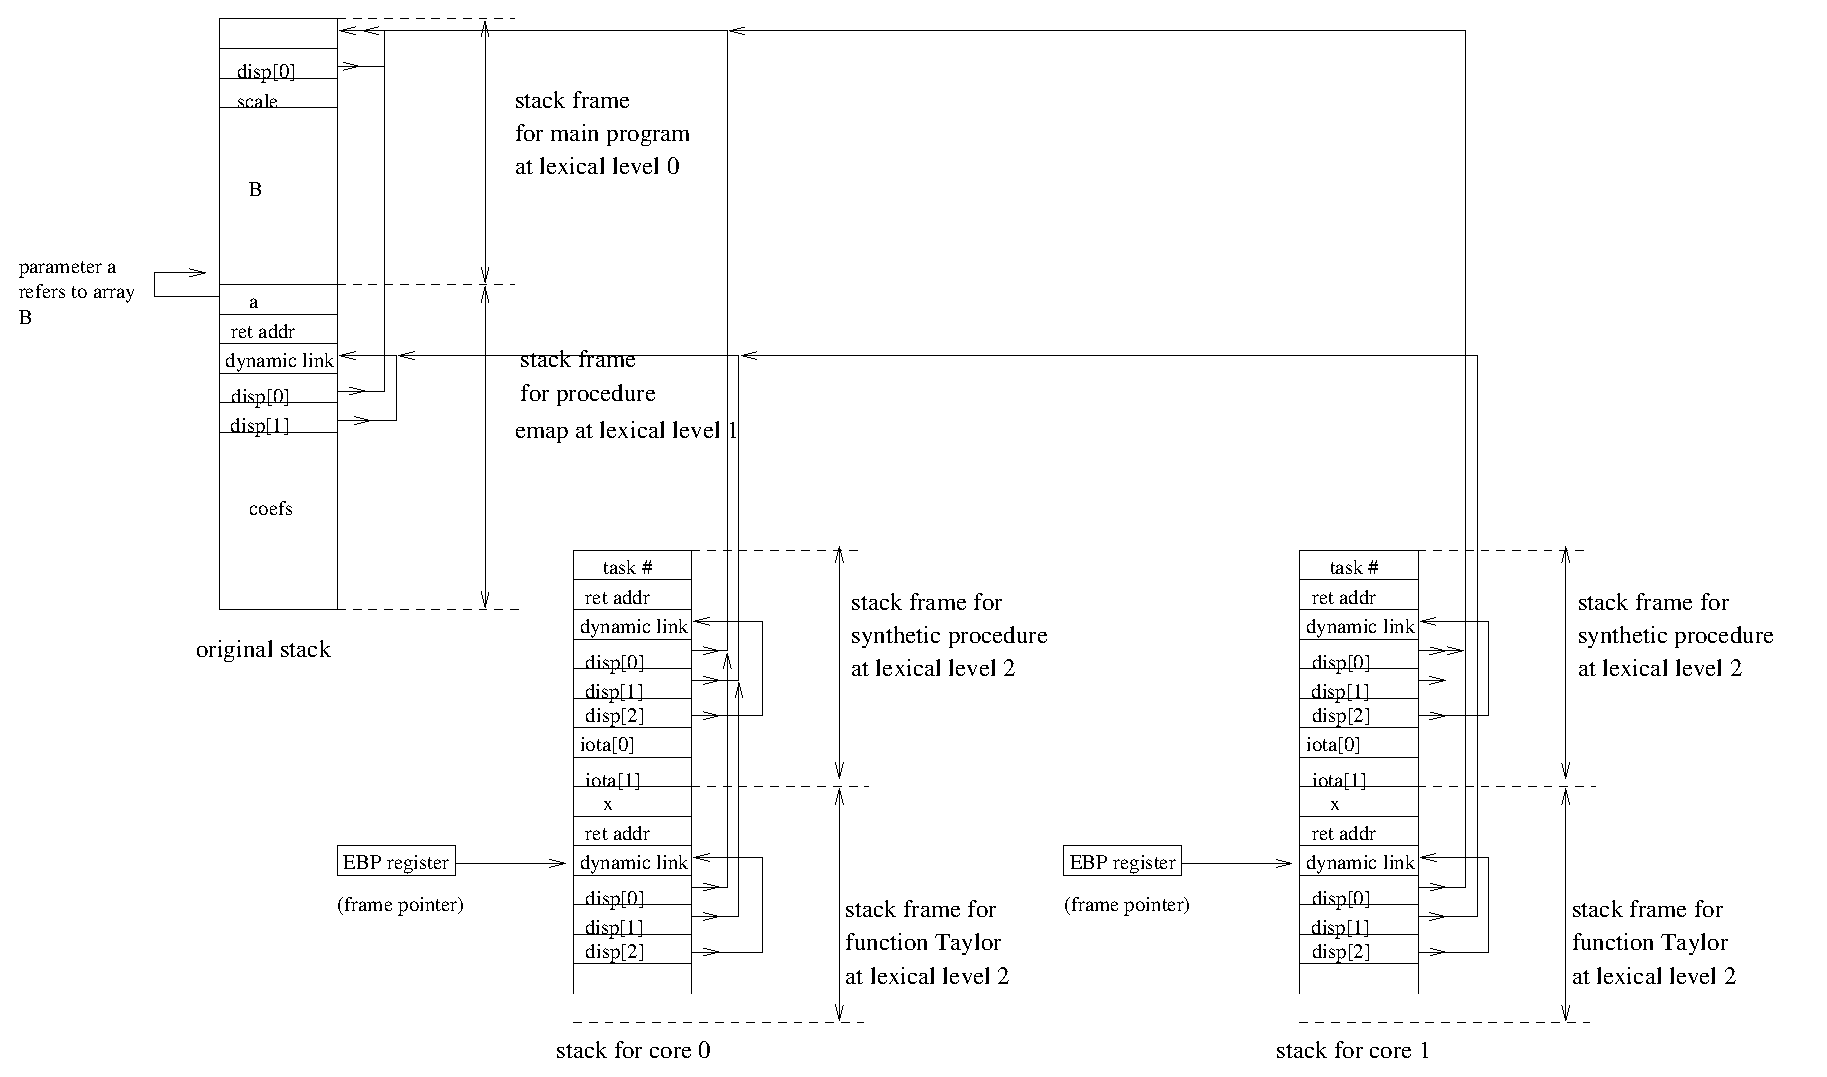
\includegraphics[scale=0.5]{nestparstack3}

\caption{The 3 stacks used by nestpar in dual core mode.\label{fig:The-3-stacks}}



\end{figure}


The function \texttt{dummy} has to run on a task stack and yet have
access to the variable \texttt{a} in \texttt{emap} and \texttt{scale}
in the main program, both of which are executing on the main stack.
It then has to call \texttt{Taylor} in such a way as to ensure that
\texttt{Taylor} can access the global \texttt{scale}. Provided that
the displays can be set up as shown in Figure \ref{fig:The-3-stacks},
this will work, but it is impossible to set up the displays this way
when using standard intel call conventions along with the \texttt{pthreads}
library. Whenever a function is executed within a thread it is allocated
a new stack that does not contain display pointers, hence variables
from containing scopes cannot be accessed.

In order to support sharing of the global stack amongst multiple tasks,
we have implemented an assembly routine \emph{taskexecute}, which
corresponds to the following C function signature:
\begin{lyxcode}
void~taskexecute(struct~threadblock~{*});
\end{lyxcode}
As can be seen, the function expects a single parameter which is a
pointer to a structure of type \emph{struct threadblock} defined as
\begin{lyxcode}
struct~threadblock\{
\begin{lyxcode}
char~{*}~savedframepointer;

char~{*}~savedcodepointer;

int~threadnumber;
\end{lyxcode}
\}
\end{lyxcode}
Above, \texttt{savedframerpointer} is the pointer to the original
stack in which the displays are already setup, \texttt{savedcodepointer}
is the pointer to the function that is being parallelised, and \texttt{threadnumber}
is a number in the range$0..n-1$ for a programme running on$n$ cores..
The following assembly code implements \texttt{taskexecute} on the
Pentium architecture.

\emph{Assembly code sequence required to implement the task execute}
\begin{lyxcode}
{\footnotesize .globl~taskexecute}{\footnotesize \par}

{\footnotesize taskexecute:}{\footnotesize \par}
\begin{lyxcode}
{\footnotesize \#~on~entry~we~have~a~pointer~in~\%esp~to~the~task~block}{\footnotesize \par}

{\footnotesize \#~this~task~block~has~the~C~definition}{\footnotesize \par}

{\footnotesize \#~struct~threadblock\{}{\footnotesize \par}

{\footnotesize \#~~~~~~~~~char~{*}~savedframepointer;}{\footnotesize \par}

{\footnotesize \#~~~~~~~~~char~{*}~savedcodepointer;}{\footnotesize \par}

{\footnotesize \#~~~~~~~~~int~threadnumber;\}}{\footnotesize \par}

{\footnotesize \#~the~first~thing~we~do~is~save~the~framepointer~on~entry}{\footnotesize \par}

{\footnotesize push~\%ebp}{\footnotesize \par}

{\footnotesize \#~next~get~the~address~of~the~stored~frame~pointer~in~the~task~block}{\footnotesize \par}

{\footnotesize mov~8(\%esp)~,~\%eax}{\footnotesize \par}

\#we~load~the~frame~pointer~into~the~hardware~frame~pointer~(ebp)

{\footnotesize mov~0(\%eax),~\%ebp}{\footnotesize \par}

{\footnotesize \#~get~the~task~number}{\footnotesize \par}

{\footnotesize push~8(\%eax)~}{\footnotesize \par}

{\footnotesize \#~make~the~call~on~the~task}{\footnotesize \par}

{\footnotesize call~{*}~4(\%eax)~}{\footnotesize \par}

{\footnotesize \#~unwind~stack~pointer}{\footnotesize \par}

{\footnotesize add~\$4,\%esp}{\footnotesize \par}

{\footnotesize \#~restore~framepointer~we~were~called~with}{\footnotesize \par}

{\footnotesize pop~\%ebp}{\footnotesize \par}

{\footnotesize ret}{\footnotesize \par}
\end{lyxcode}
\end{lyxcode}
The essence of this form of implementation is that the pthread is
setup to execute \texttt{taskexecute} which is passed \texttt{threadblock}
from the calling environment that contains the stack pointer used
by the calling environment. \texttt{taskexecute} substitutes the stack
allocated by the pthread library with the above stack before executing
the code sequence contained in the \texttt{savedcodepointe}\emph{r.}
The effect of substituting the stack pointer is undone once the called
code sequence halts to ensure a clean exit of the wrapper.


\section{Example Programs}


\subsection{Image convolution}

The first example we will look at is the use of a seperable convolution
kernel to blur an image. Convolution of an image by a matrix of real
numbers can be used to smooth or sharpen an image, depending on the
matrix used. If $A$ is an output image, $K$ a convolution matrix,
then if $B$ is the convolved image \[
B_{y,x}=\sum_{i}\sum_{j}A_{y+i,x+j}K_{i,j}\]
 

A separable convolution kernel is a vector of real numbers that can
be applied independently to the rows and columns of an image to provide
filtering. It is a specialisation of the more general convolution
matrix, but is algorithmically more efficient to implement. We can
do a seperable convolution provided that the kernel is formed by the
outer product of two vectors \textbf{a},\textbf{b}. A symmetric separable
convolution can be done if $\mathbf{a}=\mathbf{b}$.

If \textbf{k} is a symmetric separable convolution vector, then the
corresponding matrix $K$ is such that $K_{i,j}={\bf k}_{i}{\bf k}_{j}$. 

Given a starting image $A$ as a two dimensional array of pixels,
and a three element kernel $c_{1},c_{2},c_{3}$, the algorithm first
forms a temporary array $T$ whose whose elements are the weighted
sum of adjacent rows $T_{y,x}=c_{1}A_{y-1,x}+c_{2}A_{y,x}+c_{3}A_{y+1,x}$.
Then in a second phase it sets the original image to be the weighted
sum of the columns of the temporary array: $A_{y,x}=c_{1}T_{y,x-1}+c_{2}T_{y,x}+c_{3}T{y,x+1}$. 

Clearly the outer edges of the image are a special case, since the
convolution is defined over the neighbours of the pixel, and the pixels
along the boundaries a missing one neighbour. A number of solutions
are available for this, but for simplicity we will perform only vertical
convolutions on the left and right edges and horizontal convolutions
on the top and bottom lines of the image. A Vector Pascal routine
to do this is given below. The source has been pretty printed in the
latex format that is automatically generated by the compiler is listing
enabled. An equivalent sequential C routine is given in Algorithm
\ref{alg:C-version-of}. 

In comparing the C and Vector Pascal, note two features which give
performance advantages to the Vector Pascal form of the algorithm.
\begin{enumerate}
\item The support for fixed point 8 bit arithmetic with the pixel type.
This allows a higher level of parallelism to be achieved since a P4
or AMD64 can in principle operate on 16 $\times$8 bit numbers with
a single instruction. Lacking these types, the C algorithm has to
use 32 bit floats. The pixel type automatically uses saturated arithmetic.
\item The data parallel form of expression of the Vector Pascal allows more
efficient optimisation of the code.
\end{enumerate}

\subsubsection{Vector Pascal convolution algorithm}

\begin{tabbing} {*}{*}{*}\={*}{*}{*}\={*}{*}{*}\={*}{*}{*}\={*}{*}{*}\={*}{*}{*}\={*}{*}{*}\={*}{*}{*}\={*}{*}{*}\={*}{*}{*}\={*}{*}{*}\={*}{*}{*}\={*}{*}{*}\=\kill
\\
 \+%
\parbox[c]{14cm}{%
\textsf{\textbf{type}} %
}\\
 %
\parbox[c]{14cm}{%
plane(rows,cols:\textsf{\textit{integer}} \textsf{)=}\textbf{ array}
\textsf{{[}0..}\textsf{\textit{rows}} \textsf{,0..}\textsf{\textit{cols}}
\textsf{{]}}\textbf{ of} \textsf{\textit{pixel}} \textsf{;}%
}\\
 \<%
\parbox[c]{14cm}{%
\textsf{\textbf{var}} %
}\\
 %
\parbox[c]{14cm}{%
\textsf{Let} \textsf{\textit{T}}\textsf{,} \textsf{\textit{l}} \textsf{$\in$\^{ }plane;}%
}\\
 %
\parbox[c]{14cm}{%
\textsf{Let} \textsf{\textit{i}} \textsf{$\in$ integer;}%
}\\
%
\parbox[c]{14cm}{%
\textsf{\textbf{begin}} %
}\\
 \end{tabbing} Allocates a temporary buffer to hold a plane, and
3 temporary buffers to hold the convolution co-ordinates as lines
of pixels. \begin{tabbing} {*}{*}{*}\={*}{*}{*}\={*}{*}{*}\={*}{*}{*}\={*}{*}{*}\={*}{*}{*}\={*}{*}{*}\={*}{*}{*}\={*}{*}{*}\={*}{*}{*}\={*}{*}{*}\={*}{*}{*}\={*}{*}{*}\=\kill
\+ \\
 %
\parbox[c]{14cm}{%
\textsf{\textbf{new}} \textsf{\textit{(}} \textsf{\textit{T}} \textsf{,}\textsf{\textit{im}}
\textsf{.}\textsf{\textit{maxrow}} \textsf{,}\textsf{\textit{im}}
\textsf{.}\textsf{\textit{maxcol}} \textsf{);}%
}\\
 %
\parbox[c]{14cm}{%
\textsf{\textbf{new}} \textsf{\textit{(}} \textsf{\textit{l}} \textsf{,3,}\textsf{\textit{im}}
\textsf{.}\textsf{\textit{maxcol}} \textsf{);}%
}\\
 %
\parbox[c]{14cm}{%
\textsf{\textit{l}}\textsf{$\uparrow${[}0{]}$\leftarrow$} \textsf{\textit{c1}}; %
}\\
 %
\parbox[c]{14cm}{%
\textsf{\textit{l}}\textsf{$\uparrow${[}1{]}$\leftarrow$} \textsf{\textit{c2}}; %
}\\
%
\parbox[c]{14cm}{%
\textsf{\textit{l}}\textsf{$\uparrow${[}2{]}$\leftarrow$} \textsf{\textit{c3}}; %
}\\
 \end{tabbing} Perform convolution on each of the planes of the
image. This has to be done with an explicit loop as array maps only
works with functions not with procedures. \begin{tabbing} {*}{*}{*}\={*}{*}{*}\={*}{*}{*}\={*}{*}{*}\={*}{*}{*}\={*}{*}{*}\={*}{*}{*}\={*}{*}{*}\={*}{*}{*}\={*}{*}{*}\={*}{*}{*}\={*}{*}{*}\={*}{*}{*}\=\kill
\+ \\
 %
\parbox[c]{14cm}{%
\textsf{\textbf{for}} \textsf{\textit{i}}\textsf{$\leftarrow$ 0}
\textsf{\textbf{to}} \textsf{\textit{im.maxplane}} \textsf{\textbf{do}}
\textsf{\textit{convpar}} \textsf{(}\textsf{\textit{im}}\textsf{$_{\textit{i}}$,}
\textsf{\textit{l}}\textsf{$\uparrow$,} \textsf{\textit{T}}\textsf{$\uparrow$);}
\{ see section \ref{sub:convpar}\}%
}\\
 \end{tabbing} This sequence frees the temporary buffers used
in the convolution process. \begin{tabbing} {*}{*}{*}\={*}{*}{*}\={*}{*}{*}\={*}{*}{*}\={*}{*}{*}\={*}{*}{*}\={*}{*}{*}\={*}{*}{*}\={*}{*}{*}\={*}{*}{*}\={*}{*}{*}\={*}{*}{*}\={*}{*}{*}\=\kill
\+ \\
 %
\parbox[c]{14cm}{%
\textsf{\textbf{dispose}} \textsf{\textit{(}} \textsf{\textit{l}}
\textsf{);}%
}\\
 %
\parbox[c]{14cm}{%
\textsf{\textbf{dispose}} \textsf{\textit{(}} \textsf{\textit{T}}
\textsf{);}%
}\\
 \<\-%
\parbox[c]{14cm}{%
\textsf{\textbf{end}} \textsf{;}%
}\\
 \end{tabbing} 


\subsubsection{convpar\label{sub:convpar}}

\label{sec:blurtime/pconvpconvpar}

\begin{tabbing} {*}{*}{*}\={*}{*}{*}\={*}{*}{*}\={*}{*}{*}\={*}{*}{*}\={*}{*}{*}\={*}{*}{*}\={*}{*}{*}\={*}{*}{*}\={*}{*}{*}\={*}{*}{*}\={*}{*}{*}\={*}{*}{*}\=\kill
%
\parbox[c]{14cm}{%
\textsf{\textbf{procedure}} \textsf{\textit{convpar}} \textsf{\textit{(}}
\textsf{\textbf{var}} \textsf{\textit{p}} \textsf{,}\textsf{\textit{l}}
\textsf{,}\textsf{\textit{T}} \textsf{:}\textsf{\textit{plane}} \textsf{);}%
}\\
 \end{tabbing} This convolves a plane by applying the vertical
and horizontal convolutions in turn. \begin{tabbing} {*}{*}{*}\={*}{*}{*}\={*}{*}{*}\={*}{*}{*}\={*}{*}{*}\={*}{*}{*}\={*}{*}{*}\={*}{*}{*}\={*}{*}{*}\={*}{*}{*}\={*}{*}{*}\={*}{*}{*}\={*}{*}{*}\=\kill
\\
 \+%
\parbox[c]{14cm}{%
\textsf{\textbf{var}} %
}\\
 %
\parbox[c]{14cm}{%
\textsf{Let} \textsf{\textit{r}}\textsf{,} \textsf{\textit{c}} \textsf{$\in$
integer;}%
}\\
 \-\<\+%
\parbox[c]{14cm}{%
\textsf{\textbf{begin}} %
}\\
 \end{tabbing} This sequence performs a vertical convolution of
the rows of the plane p and places the result in the temporary plane
$T$. It uses the lines of pixels \textsf{l{[}i{]}} as convolution
weights. Use of lines of pixels rather than the floating point numbers
for the kernel weights allows the computation to proceed 8 pixels
at a time in parallel. The lines \textsf{\textit{T}}\textsf{$_{0}$$\leftarrow$}
\textsf{\textit{p}}\textsf{$_{0}$}; and \textsf{\textit{T}}\textsf{$_{\textit{r}}$$\leftarrow$}
\textsf{\textit{p}}\textsf{$_{\textit{r}}$}; deal with the top and
bottom rows of the picture which are left unchanged.

\begin{tabbing} {*}{*}{*}\={*}{*}{*}\={*}{*}{*}\={*}{*}{*}\={*}{*}{*}\={*}{*}{*}\={*}{*}{*}\={*}{*}{*}\={*}{*}{*}\={*}{*}{*}\={*}{*}{*}\={*}{*}{*}\={*}{*}{*}\=\kill
\+ \\
 %
\parbox[c]{14cm}{%
\texttt{\small {\{\$r-\}\{disable range checks\}}}%
}\\
 %
\parbox[c]{14cm}{%
\textsf{\textit{r}}\textsf{$\leftarrow$} \textsf{\textit{p.rows}}; %
}\\
 %
\parbox[c]{14cm}{%
\textsf{\textit{T}}\textsf{$_{1..\textit{r}-1}$$\leftarrow$} \textsf{\textit{p}}\textsf{$_{0..\textit{r}-2}$
$\times$} \textsf{\textit{l}}\textsf{$_{0}$ +} \textsf{\textit{p}}\textsf{$_{1..\textit{r}-1}$
$\times$} \textsf{\textit{l}}\textsf{$_{1}$ +} \textsf{\textit{p}}\textsf{$_{2..\textit{r}}$
$\times$} \textsf{\textit{l}}\textsf{$_{2}$}; %
}\\
 %
\parbox[c]{14cm}{%
\textsf{\textit{T}}\textsf{$_{0}$$\leftarrow$} \textsf{\textit{p}}\textsf{$_{0}$}; %
}\\
 %
\parbox[c]{14cm}{%
\textsf{\textit{T}}\textsf{$_{\textit{r}}$$\leftarrow$} \textsf{\textit{p}}\textsf{$_{\textit{r}}$}; %
}\\
 \end{tabbing} Now perform a horizontal convolution of the plane
$T$ and place the result in p. \begin{tabbing} {*}{*}{*}\={*}{*}{*}\={*}{*}{*}\={*}{*}{*}\={*}{*}{*}\={*}{*}{*}\={*}{*}{*}\={*}{*}{*}\={*}{*}{*}\={*}{*}{*}\={*}{*}{*}\={*}{*}{*}\={*}{*}{*}\=\kill
\+ \\
 %
\parbox[c]{14cm}{%
\textsf{\textit{c}}\textsf{$\leftarrow$} \textsf{\textit{p.cols}}; %
}\\
 %
\parbox[c]{14cm}{%
\textsf{\textit{p}}\textsf{$_{0..\textit{r},1..\textit{c}-1}$$\leftarrow$}
\textsf{\textit{T}}\textsf{$_{0..\textit{r},0..\textit{c}-2}$ $\times$}
\textsf{\textit{l}}\textsf{$_{0}$ +} \textsf{\textit{T}}\textsf{$_{0..\textit{r},2..\textit{c}}$
$\times$} \textsf{\textit{l}}\textsf{$_{2}$ +} \textsf{\textit{T}}\textsf{$_{0..\textit{r},1..\textit{c}-1}$
$\times$} \textsf{\textit{l}}\textsf{$_{1}$}; %
}\\
 %
\parbox[c]{14cm}{%
\textsf{\textit{p}}\textsf{$_{0..\textit{r},0}$$\leftarrow$} \textsf{\textit{T}}\textsf{$_{0..\textit{r},0}$}; %
}\\
 %
\parbox[c]{14cm}{%
\textsf{\textit{p}}\textsf{$_{0..\textit{r},\textit{c}}$$\leftarrow$}
\textsf{\textit{T}}\textsf{$_{0..\textit{r},\textit{c}}$}; %
}\\
 %
\parbox[c]{14cm}{%
\texttt{\small {\{\$r+\}\{enable range checks\}}}%
}\\
 \\
 \<\-%
\parbox[c]{14cm}{%
\textsf{\textbf{end}} \textsf{;}%
}\\
 \end{tabbing} 

%
\begin{algorithm}


\caption{C version of the convolution routine.\label{alg:C-version-of}}

\begin{lyxcode}
\#include~<stdlib.h>

conv(char~{*}im,~int~planes,~int~rows,int~cols,float~c1,float~c2,float~c3)

/{*}~C~version~of~a~convolution~routine~{*}/

\{~

~int~i,j,p,temp;

~int~planestep=rows{*}cols;

~char~{*}~plane,~{*}~buffplane;

~char~{*}~buff~=~malloc(~rows{*}planes{*}cols);

~for~(p=0;p<planes;p++)\{

~~plane~=~\&im{[}p{*}planestep{]};

~~buffplane=~\&buff{[}p{*}planestep{]};

~~/{*}~convolve~horizontally~{*}/

~~for(i=0;i<rows;i++)\{

~~~for(j=1;j<(cols-1);j++)~\{

~~~~temp=~plane{[}i{*}cols+j-1{]}{*}c1+plane{[}i{*}cols+j{]}{*}c2+plane{[}i{*}cols+j+1{]}{*}c3;

~~~~if~(temp<0)\{temp=0;\}

~~~~else~if~(temp>255)~\{~temp=255;\}~;

~~~~buffplane{[}i{*}cols+j{]}=temp;

~~~\}

~~~buffplane{[}i{*}cols{]}=plane{[}i{*}cols{]};

~~~buffplane{[}i{*}cols+cols-1{]}=plane{[}i{*}cols+cols-1{]};

~~\}

/{*}~convolve~vertically~{*}/

~~for(j=0;j<cols;j++)~\{

~~~for(i=1;i<rows-1;i++)\{

~~~~temp=~buffplane{[}(i-1){*}cols+j{]}{*}c1+buffplane{[}i{*}cols+j{]}{*}c2+buffplane{[}(1+i){*}cols+j{]}{*}c3;

~~~~if(temp<0)\{temp=0;\}

~~~~else~if~(temp>255)~\{~temp=255;\}~;

~~~~plane{[}i{*}cols+j{]}=temp;

~~~\}

~~~plane{[}j{]}=buffplane{[}j{]};

~~~plane{[}(rows-1){*}cols+j{]}=buffplane{[}~(rows-1){*}cols+j{]};

~~\}

~\}

~free(buff);

\}
\end{lyxcode}

\end{algorithm}



\subsection{Performance comparisons}

%
\begin{figure}
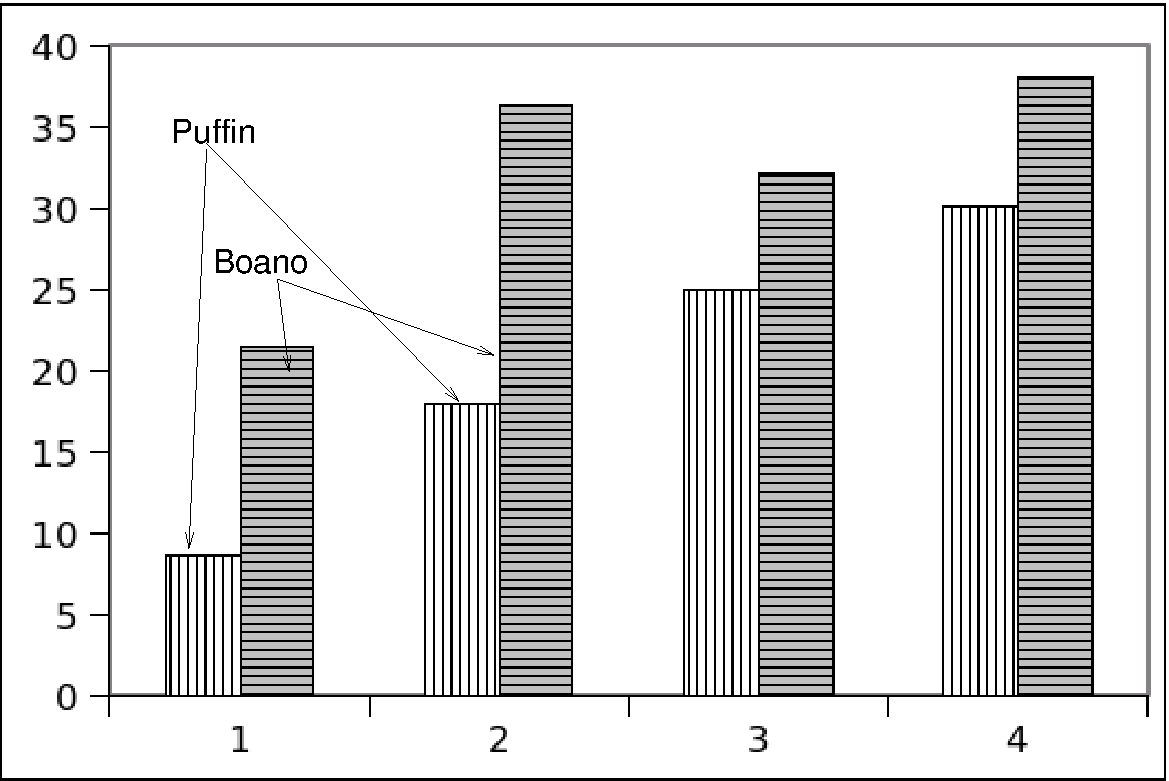
\includegraphics[scale=0.4]{boanopuffin}

\caption{Comparison of perfomance gains over the sequential C implementation
of the convolution routine on different processors and numbers of
cores. The x-axis shows the number of cores for which the program
was compiled, the y-axis shows the the relative speedup. Puffin has
4x Quad-Core AMD Opteron 8350 Processor chips running the AMD64 instruction
set with a CPU clock of 1Ghz. Boano has 4x Single-Core Intel Xeon
CPUs at 2.80GHz running the 32 bit Intel P4 instructions. In each
case the performance is normalised so that the speed of the C code
counts as 1.\label{fig:Comparison-of-perfomance} }



\end{figure}


%
\begin{table}[h]
\caption{Data used to produce Figure \ref{fig:Comparison-of-perfomance}. It
gives the times in seconds to perform 30 convolutions on a 1024$\times$1024
pixel image with 24 bits per pixel, organised as 3 distinct colour
planes, whilst using a 3 element separable kernel. \label{tab:Data-used-to}}


%%%%%%%%%%%%%%%%%%%%%%%%%%%%%%%%%%%%%%%%%%%%%%%%%%%%%%%%%%%%%%%%%%%%%% %%                                                                  %% %%  This is a LaTeX2e table fragment exported from Gnumeric.        %% %%                                                                  %% %%%%%%%%%%%%%%%%%%%%%%%%%%%%%%%%%%%%%%%%%%%%%%%%%%%%%%%%%%%%%%%%%%%%%%
\begin{tabular}{l|r|rrrrrr}\hline
&gcc	&vpc	&	&	&\\
cores	& 1	&1  	&2  	&3  	&4 &8&16\\
	\hline\hline Machine\\\hline
Puffin	&5.48	&0.81	&0.39	&0.28	&0.23&0.18&0.16\\ Boano	&23.02	&1.07	&0.63	&0.72	&0.60\\\hline
\end{tabular}


\end{table}


We give examples of running the two algorithms on both 32bit and 64bit
multi-core machines. Results are summarised in Figure \ref{fig:Comparison-of-perfomance}
and Table \ref{tab:Data-used-to}. In all cases the algorithms were
compiled at the optimisation level 0 for both compilers. 

As would be expected the parallel version of the algorithm significantly
out-performs the sequential version. However it is clear that SIMD
parallelism provides a more reliable form of acceleration than MIMD.
The initial speedup figures using a single core rely entirely on the
use of SIMD instructions. SIMD alone gives an acceleration of over
$8\times$ on an Opteron and $21\times$on a Xeon. The gain from MIMD
is more modest and tails off after markedly after 2 processors on
Boano, and after 3 processors on Puffin. This result is consistent
with the SIMD code, which operates on wide words, saturating the available
memory bandwidth.


\subsection{Mandelbrot set}

It is perhaps not surprising that the image convolution example gives
very favourable results for parallel code. This was, after all, what
Intel designed the MMX instruction set to do. The next case we look
at is computing the Mandelbrot set. Strictly, this is defined as the
set of complex numbers $M$ such that for all $c\in M$ the sequence
$z_{0}=c,z_{n+1}=z_{n}^{2}+c$ does not diverge, i.e, $|z_{n}|<k$
for some $k>1$. %
\begin{figure}

\includegraphics[width=12cm]{mandel1b}

\caption{The Mandelbrot set image\label{fig:The-Mandelbrot-set-iimage} produced
by Algorithm \ref{alg:MIMD-version-of}. The original file produced
by the algorithm is 4 megabytes in size. Note that since the type
Pixel is a signed 8 bit number, 0 translates to mid grey. We have
limited ourselves to this rather dull rendering to make the rendering
procedure more readily understandable.}



\end{figure}
 %
\begin{algorithm}
\caption{Escape time computed by a sequential ISO-Pascal routine using complex
numbers.\label{alg:Escape-time-computed}}


\begin{tabbing} {*}{*}{*}\={*}{*}{*}\={*}{*}{*}\={*}{*}{*}\={*}{*}{*}\={*}{*}{*}\={*}{*}{*}\={*}{*}{*}\={*}{*}{*}\={*}{*}{*}\={*}{*}{*}\={*}{*}{*}\={*}{*}{*}\=\kill
%
\parbox[c]{14cm}{%
\textsf{\textbf{function}} \textsf{\textit{escapebrightness}} \textsf{\textit{(}}
\textsf{\textit{c}} \textsf{:} \textsf{\textit{complex}} \textsf{):}\textsf{\textit{real}}
\textsf{;}%
}\\
 %
\parbox[c]{14cm}{%
\textsf{\textbf{label}} \textsf{99;}%
}\\
 \+%
\parbox[c]{14cm}{%
\textsf{\textbf{var}} %
}\\
 %
\parbox[c]{14cm}{%
\textsf{Let} \textsf{\textit{z}} \textsf{$\in$ complex;}%
}\\
 %
\parbox[c]{14cm}{%
\textsf{Let} \textsf{\textit{i}} \textsf{$\in$ integer;}%
}\\
 \-\<\+%
\parbox[c]{14cm}{%
\textsf{\textbf{begin}} %
}\\
 %
\parbox[c]{14cm}{%
\textsf{\textit{z}}\textsf{$\leftarrow$ 0.0}; %
}\\
 \+%
\parbox[c]{14cm}{%
\textsf{\textbf{for}} \textsf{\textit{i}}\textsf{$\leftarrow$} \textsf{\textit{escapelimit}}
\textsf{\textbf{downto}} \textsf{1} \textsf{\textbf{do}} %
}\\
 \<%
\parbox[c]{14cm}{%
\textsf{\textbf{begin}} %
}\\
 %
\parbox[c]{14cm}{%
\textsf{\textit{z}}\textsf{$\leftarrow$} \textsf{\textit{z}} \textsf{$\times$}
\textsf{\textit{z}} \textsf{+} \textsf{\textit{c}}; %
}\\
 \+%
\parbox[c]{14cm}{%
\textsf{\textbf{if}} \textsf{\textit{escaped}} \textsf{(}\textsf{\textit{z}}\textsf{)}
\textsf{\textbf{then}} %
}\\
 \<%
\parbox[c]{14cm}{%
\textsf{\textbf{begin}} %
}\\
 %
\parbox[c]{14cm}{%
\textsf{\textit{escapebrightness}}\textsf{$\leftarrow$} \textsf{\textit{i}}
\textsf{$\times$} \textsf{\textit{pixelshift}}; %
}\\
 %
\parbox[c]{14cm}{%
\textsf{\textbf{goto}} \textsf{99;} %
}\\
 \<\-%
\parbox[c]{14cm}{%
\textsf{\textbf{end}} \textsf{;}%
}\\
 \<\-%
\parbox[c]{14cm}{%
\textsf{\textbf{end}} \textsf{;}%
}\\
 %
\parbox[c]{14cm}{%
\textsf{\textit{escapebrightness}}\textsf{$\leftarrow$ 0}; %
}\\
 %
\parbox[c]{14cm}{%
99:\textsf{;}%
}\\
 \<\-%
\parbox[c]{14cm}{%
\textsf{\textbf{end}} \textsf{;}%
}\\
 \end{tabbing}

\begin{tabbing} {*}{*}{*}\={*}{*}{*}\={*}{*}{*}\={*}{*}{*}\={*}{*}{*}\={*}{*}{*}\={*}{*}{*}\={*}{*}{*}\={*}{*}{*}\={*}{*}{*}\={*}{*}{*}\={*}{*}{*}\={*}{*}{*}\=\kill
%
\parbox[c]{14cm}{%
\textsf{\textbf{procedure}} \textsf{\textit{buildpic}} \textsf{\textit{(}}
\textsf{\textbf{var}} \textsf{\textit{p}} \textsf{:}\textsf{\textit{picture}}
\textsf{);}%
}\\
 \+%
\parbox[c]{14cm}{%
\textsf{\textbf{var}} %
}\\
 %
\parbox[c]{14cm}{%
\textsf{Let} \textsf{\textit{x}}\textsf{,} \textsf{\textit{y}} \textsf{$\in$
integer;}%
}\\
 \-\<\+%
\parbox[c]{14cm}{%
\textsf{\textbf{begin}} %
}\\
 \+%
\parbox[c]{14cm}{%
\textsf{\textbf{for}} \textsf{\textit{x}}\textsf{$\leftarrow$ 0}
\textsf{\textbf{to}} \textsf{\textit{imlim}} \textsf{\textbf{do}} %
}\\
 \+%
\parbox[c]{14cm}{%
\textsf{\textbf{for}} \textsf{\textit{y}}\textsf{$\leftarrow$ 0}
\textsf{\textbf{to}} \textsf{\textit{imlim}} \textsf{\textbf{do}} %
}\\
 \-\-%
\parbox[c]{14cm}{%
\textsf{\textit{p}}\textsf{$_{\textit{y},\textit{x}}$$\leftarrow$}
\textsf{\textit{escapebrightness}} \textsf{(}\textsf{\textit{cmplx}}
\textsf{(}\textsf{\textit{xorigin}} \textsf{+} \textsf{\textit{xstep}}
\textsf{$\times$} \textsf{\textit{x}}\textsf{,} \textsf{\textit{yorigin}}
\textsf{+} \textsf{\textit{ystep}} \textsf{$\times$} \textsf{\textit{y}}\textsf{))}; %
}\\
 \<\-%
\parbox[c]{14cm}{%
\textsf{\textbf{end}} \textsf{;}%
}\\
 \end{tabbing} 
\end{algorithm}


%
\begin{algorithm}
\caption{MIMD Vector Pascal version of Algorithm \ref{alg:Escape-time-computed}
using real arithmetic.\label{alg:MIMD-version-of}}


\begin{tabbing} {*}{*}{*}\={*}{*}{*}\={*}{*}{*}\={*}{*}{*}\={*}{*}{*}\={*}{*}{*}\={*}{*}{*}\={*}{*}{*}\={*}{*}{*}\={*}{*}{*}\={*}{*}{*}\={*}{*}{*}\={*}{*}{*}\=\kill
\\
 \+ \\
\< %
\parbox[c]{14cm}{%
\textsf{\textbf{pure}} \textsf{\textbf{function}} \textsf{\textit{escapebrightness}}
\textsf{(}\textsf{\textit{cx}}\textsf{,} \textsf{\textit{cy}} \textsf{:}
\textsf{\textit{real}}\textsf{) :} \textsf{\textit{real}}; %
}\\
 %
\parbox[c]{14cm}{%
\textsf{\textbf{label}} \textsf{99 ;}%
}\\
 \<%
\parbox[c]{14cm}{%
\textsf{\textbf{var}} %
}\\
 %
\parbox[c]{14cm}{%
\textsf{Let} \textsf{\textit{xx}}\textsf{,} \textsf{\textit{y}}\textsf{,}
\textsf{\textit{x}}\textsf{,} \textsf{\textit{x2}}\textsf{,} \textsf{\textit{y2}}
\textsf{$\in$ real;}%
}\\
 %
\parbox[c]{14cm}{%
\textsf{Let} \textsf{\textit{iteration}} \textsf{$\in$ integer;}%
} \\
 \-\<\+%
\parbox[c]{14cm}{%
\textsf{\textbf{begin}} %
}\\
 %
\parbox[c]{14cm}{%
\textsf{\textit{x}}\textsf{$\leftarrow$ 0.0}; %
}\\
 %
\parbox[c]{14cm}{%
\textsf{\textit{y}}\textsf{$\leftarrow$ 0.0}; %
}\\
 %
\parbox[c]{14cm}{%
\textsf{\textit{iteration}}\textsf{$\leftarrow$ 1}; %
}\\
 \+%
\parbox[c]{14cm}{%
\textsf{\textbf{while}} \textsf{\textit{iteration}} \textsf{$<$}
\textsf{\textit{escapelimit}} \textsf{\textbf{do}} %
}\\
 \<%
\parbox[c]{14cm}{%
\textsf{\textbf{begin}} %
}\\
 %
\parbox[c]{14cm}{%
\textsf{\textit{xx}}\textsf{$\leftarrow$ (}\textsf{\textit{x}}\textsf{)$^{2}$
- (}\textsf{\textit{y}}\textsf{)$^{2}$ +} \textsf{\textit{cx}}; %
}\\
 %
\parbox[c]{14cm}{%
\textsf{\textit{y}}\textsf{$\leftarrow$ 2.0 $\times$} \textsf{\textit{x}}
\textsf{$\times$} \textsf{\textit{y}} \textsf{+} \textsf{\textit{cy}}; %
}\\
 %
\parbox[c]{14cm}{%
\textsf{\textit{x}}\textsf{$\leftarrow$} \textsf{\textit{xx}}; %
}\\
 \+%
\parbox[c]{14cm}{%
\textsf{\textbf{if}} \textsf{(((}\textsf{\textit{x}}\textsf{)$^{2}$
+ (}\textsf{\textit{y}}\textsf{)$^{2}$) $>$} \textsf{\textit{escapebound}}\textsf{)}
\textsf{\textbf{then}} %
}\\
 \-%
\parbox[c]{14cm}{%
\textsf{\textbf{goto}} \textsf{99;} %
}\\
 %
\parbox[c]{14cm}{%
\textsf{\textit{iteration}}\textsf{$\leftarrow$} \textsf{\textit{iteration}}
\textsf{+ 1}; %
}\\
 \<\-%
\parbox[c]{14cm}{%
\textsf{\textbf{end}} \textsf{;}%
}\\
 \+%
\parbox[c]{14cm}{%
99:\textbf{ if} \textsf{\textit{iteration}} \textsf{$<$} \textsf{\textit{escapelimit}}\textbf{
then} \textsf{\textit{escapebrightness}}\textsf{$\leftarrow$} \textsf{\textit{iteration}}
\textsf{$\times$} \textsf{\textit{pixelshift}}%
}\\
 \-\<%
\parbox[c]{14cm}{%
\textsf{\textbf{else}} \textsf{\textit{escapebrightness}}\textsf{$\leftarrow$
0.0;} %
}\\
 \<\-%
\parbox[c]{14cm}{%
\textsf{\textbf{end}} \textsf{;}%
}\\
 \end{tabbing} 

\label{sec:mandelbrot1bbuildpic}

\begin{tabbing} {*}{*}{*}\={*}{*}{*}\={*}{*}{*}\={*}{*}{*}\={*}{*}{*}\={*}{*}{*}\={*}{*}{*}\={*}{*}{*}\={*}{*}{*}\={*}{*}{*}\={*}{*}{*}\={*}{*}{*}\={*}{*}{*}\=\kill
%
\parbox[c]{14cm}{%
\textsf{\textbf{procedure}} \textsf{\textit{buildpic}} \textsf{\textit{(}}
\textsf{\textbf{var}} \textsf{\textit{p}} \textsf{:}\textsf{\textit{picture}}
\textsf{);}%
}\\
 \+%
\parbox[c]{14cm}{%
\textsf{\textbf{var}} %
}\\
 %
\parbox[c]{14cm}{%
\textsf{Let} \textsf{\textit{x}}\textsf{,} \textsf{\textit{y}} \textsf{$\in$
integer;}%
}\\
 \-\<\+%
\parbox[c]{14cm}{%
\textsf{\textbf{begin}} %
}\\
 %
\parbox[c]{14cm}{%
\textsf{\textit{p}}\textsf{$\leftarrow$} \textsf{\textit{escapebrightness}}
\textsf{(}\textsf{\textit{xorigin}} \textsf{+} \textsf{\textit{xstep}}
\textsf{$\times$} \textsf{$\iota{}_{1}$,} \textsf{\textit{yorigin}}
\textsf{+} \textsf{\textit{ystep}} \textsf{$\times$} \textsf{$\iota{}_{0}$)}; %
}\\
 \<\-%
\parbox[c]{14cm}{%
\textsf{\textbf{end}} \textsf{;}%
}\\
 \end{tabbing} 
\end{algorithm}
%
\begin{algorithm}
\caption{Version of the Mandelbrot\label{alg:Version-of-the} algorithm that
exploits both SIMD and MIMD parallelism. In this, the variables \textsf{\textsl{x,
y, cx, cy, times}} are all arrays rather than scalars.}


\begin{tabbing} {*}{*}{*}\={*}{*}{*}\={*}{*}{*}\={*}{*}{*}\={*}{*}{*}\={*}{*}{*}\={*}{*}{*}\={*}{*}{*}\={*}{*}{*}\={*}{*}{*}\={*}{*}{*}\={*}{*}{*}\={*}{*}{*}\=\kill
%
\parbox[c]{14cm}{%
\textsf{\textbf{procedure}} \textsf{\textit{buildpic}} \textsf{\textit{(}}
\textsf{\textbf{var}} \textsf{\textit{p}} \textsf{:}\textsf{\textit{picture}}
\textsf{);}%
}\\
 \+%
\parbox[c]{14cm}{%
\textsf{\textbf{var}} %
}\\
 %
\parbox[c]{14cm}{%
\textsf{Let} \textsf{\textit{iteration}} \textsf{$\in$ integer;}%
}\\
 \\
 \-\<\+%
\parbox[c]{14cm}{%
\textsf{\textbf{begin}} %
}\\
 %
\parbox[c]{14cm}{%
\textsf{\textit{x}}\textsf{$\leftarrow$ 0.0}; %
}\\
 %
\parbox[c]{14cm}{%
\textsf{\textit{y}}\textsf{$\leftarrow$ 0.0}; %
}\\
 %
\parbox[c]{14cm}{%
\textsf{\textit{cx}}\textsf{$\leftarrow$} \textsf{\textit{xorigin}}
\textsf{+} \textsf{\textit{xstep}} \textsf{$\times$} \textsf{\textit{iota}}\textsf{$_{1}$}; %
}\\
 %
\parbox[c]{14cm}{%
\textsf{\textit{cy}}\textsf{$\leftarrow$} \textsf{\textit{yorigin}}
\textsf{+} \textsf{\textit{ystep}} \textsf{$\times$} \textsf{\textit{iota}}\textsf{$_{0}$}; %
}\\
 %
\parbox[c]{14cm}{%
\textsf{\textit{times}}\textsf{$\leftarrow$ 0}; %
}\\
 \+%
\parbox[c]{14cm}{%
\textsf{\textbf{for}} \textsf{\textit{iteration}}\textsf{$\leftarrow$
1} \textsf{\textbf{to}} \textsf{\textit{escapelimit}} \textsf{\textbf{do}} %
}\\
 \<%
\parbox[c]{14cm}{%
\textsf{\textbf{begin}} %
}\\
 %
\parbox[c]{14cm}{%
\textsf{\textit{xx}}\textsf{$\leftarrow$} \textsf{\textit{x}} \textsf{$\times$}
\textsf{\textit{x}} \textsf{-} \textsf{\textit{y}} \textsf{$\times$}
\textsf{\textit{y}} \textsf{+} \textsf{\textit{cx}}; %
}\\
 %
\parbox[c]{14cm}{%
\textsf{\textit{y}}\textsf{$\leftarrow$ 2.0 $\times$} \textsf{\textit{x}}
\textsf{$\times$} \textsf{\textit{y}} \textsf{+} \textsf{\textit{cy}}; %
}\\
 %
\parbox[c]{14cm}{%
\textsf{\textit{x}}\textsf{$\leftarrow$} \textsf{\textit{xx}}; %
}\\
 \+%
\parbox[c]{14cm}{%
\textsf{\textit{times}} \textsf{$\leftarrow$} \textsf{\textbf{if}}
\textsf{\textit{times}} \textsf{=0} \textsf{\textbf{then}} %
}\\
 \+%
\parbox[c]{14cm}{%
\textsf{\textbf{if}} \textsf{(}\textsf{\textit{x}} \textsf{$\times$}
\textsf{\textit{x}} \textsf{+} \textsf{\textit{y}} \textsf{$\times$}
\textsf{\textit{y}} \textsf{$>$} \textsf{\textit{escapebound}}\textsf{)}
\textsf{\textbf{then}} \textsf{\textit{iteration}} \textsf{\textbf{else}}
\textsf{0}%
}\\
 \-\<%
\parbox[c]{14cm}{%
\textsf{\textbf{else}} \textsf{\textit{times}}\textsf{;} %
}\\
 \\
 \<\-\<\-%
\parbox[c]{14cm}{%
\textsf{\textbf{end}} \textsf{;}%
}\\
 \\
 %
\parbox[c]{14cm}{%
\textsf{\textit{p}}\textsf{$\leftarrow$} \textsf{\textit{times}}
\textsf{$\times$} \textsf{\textit{pixelshift}}; %
}\\
 \<\-%
\parbox[c]{14cm}{%
\textsf{\textbf{end}} \textsf{;}%
}\\
 \end{tabbing} 
\end{algorithm}


To generate a pretty picture like Figure \ref{fig:The-Mandelbrot-set-iimage},
one typically plots the complex plane and for each pixel position
one computes the number of iterations it takes for the formula to
diverge. The divergence time is then used to define the colour or
brightness of a pixel. The problem is potentially highly parallel,
since the divergence time of each point is independent of all other
points. On closer examination though we find that the sort of parallelism
is not one readily amenable to SIMD evaluation. To understand this
look at Algorithms \ref{alg:Escape-time-computed} and \ref{alg:MIMD-version-of}. 

Algorithm \ref{alg:Escape-time-computed} is a simple sequential algorithm
which is directly based on the definition of the Mandelbrot set. The
core of the algorithm is the function \textsf{\textit{escapebrightness}}
which for the complex number given by \textsf{\textit{c}} will compute
the number of iterations required for divergence to occur. The picture
is then built up by the procedure \textsf{\textit{buildpic}} which
uses nested loops to call for the complex number corresponding to
each pixel position. This algorithm ran in 378 seconds to compute
the set to a resolution of 2048 pixels square.

%
\begin{table}
\caption{Timings in seconds for Mandelbrot algorithms computing the Mandelbrot
set at 2048$\times$2048 resolution on the quad Intel Xeon processor
Boano.\label{tab:Timings-for-Mandelbrot} Pascal algorithms as numbered
in the chapter. The Fortran95 version is almost the same as Algorithm
\ref{alg:MIMD-version-of} apart from superficial language differences.
It is compiled with an research Fortran95 compiler written by Paul
Keir at the University of Glasgow. The C version is mandelbrot-1.c
written by Michael Ashley, University of New South Wales.}


\begin{tabular}{|c|c|c|c|c|c|}
\hline 
Algorithm & \ref{alg:Escape-time-computed} & \ref{alg:MIMD-version-of} & \ref{alg:Version-of-the} & Fortran95 & C\tabularnewline
\hline
Cores &  &  &  &  & \tabularnewline
1 & 378 & 10.3 & 187 & 10.7 & 10.2\tabularnewline
2 &  & 5.6 &  & 5.8 & \tabularnewline
3 &  & 4.5 & 91 & 4.6 & \tabularnewline
4 &  & 3.7 & 82 & 3.9 & \tabularnewline
\hline
\end{tabular}
\end{table}


We then try and speed this up in Algorithm \ref{alg:MIMD-version-of}
by applying two transformations.
\begin{enumerate}
\item We replaced the use of complex numbers by reals. This can be expected
to accelerate things as complex arithmetic is implemented with calls
to a library. This is an inelegant but effective accelerator. Table
\ref{tab:Timings-for-Mandelbrot} shows an acceleration from 378 seconds
to 10.3 
\item We replaced the sequential loops in\textsf{\textit{ buildpic}} with
an implicit map. This will allow parallelism provided that we have
qualified\textsf{\textit{ escapebrightness}} as a pure function. This
allows the algorithm to be accelerated by a further factor of about
3 when when compiled for 4 cores. 
\end{enumerate}
Table \ref{tab:Timings-for-Mandelbrot} shows very similar timings
for C, Vector Pascal and Fortran95 for the single core case. Since
the file formats generated for the final image differ between implementations,
the differences in timings are not significant. The multi-core acceleration
achieved by the Fortran95 and Vector Pascal versions are also essentially
the same.

One might hope that it should be possible to gain another factor of
4 in performance by taking advantage of the fact that a P4 class processor
can handle 4 floating point numbers at a time. However a SIMD version
of the algorithm runs into problems since it must be cast in a form
that allows the same operations to be performed simultaneously on
a number of data points. But the divergence time will differ between
different positions on the complex plane, which makes it difficult
to compute several points in lockstep. When one point has already
diverged, others have not. Thus we can not have the loop breakout
used in the earlier algorithms. Algorithm \ref{alg:Version-of-the}
shows how the problem can be expressed in SIMD fashion, operating
in lockstep on all points in the complex plane. A conditional expression
is now used to gather the escape times. These can be executed in SIMD
fashion with no branches.

The performance of the SIMD version is frankly disappointing as shown
in Table \ref{tab:Timings-for-Mandelbrot}. It runs in about 1/20th
the speed of the MIMD version. This can be explained by the fact that
most of the points being examined on the complex plane will diverge
rapidly, a great deal of wasted computation is done because the SIMD
version can not exploit this. A second factor will be the much poorer
cache usage because each statement uses 2D arrays that are too big
to fit in the cache. 


\section{Conclusion}

Modern desktop computers have the potential to perform highly parallel
computations. But realising this potential remains tricky. Array languages
like Vector Pascal, SAC or Fortran95 are one promising approach. Highest
performance is attained when one can utilise both the SIMD and the
MIMD potential of modern chips. This not only requires a compiler
that is able to target both forms of parallelism but also requires
an appropriate problem domain. Even problems which, on first sight,
are highly parallel, may not lend themselves to both sorts of parallelism.
But when both SIMD and MIMD can be harnessed, the performance gains
are startling.
\begin{lyxcode}
~
\end{lyxcode}
\bibliographystyle{plain}
\bibliography{database}

\end{document}
